\documentclass[reqno,12pt,notitlepage]{article}

\usepackage{pdfpages}
\usepackage{amsmath}
\usepackage{amsthm}
\usepackage{amssymb}
\usepackage{setspace}
\usepackage{graphicx}
\usepackage{booktabs}
\usepackage{pdflscape}
\usepackage{url}
\usepackage{caption}
\usepackage{multirow,rotating,multicol}
\usepackage{listings}
\usepackage{longtable}
\usepackage{threeparttable}
\usepackage{subcaption}
\usepackage{float}
\usepackage{pgfpages,tikz}
\usepackage{adjustbox}
\usepackage{enumitem}
\usepackage{appendix}
\usepackage{dsfont}
\usepackage{natbib}
\usepackage{bookmark}
\usepackage[utf8]{inputenc}
\usepackage{textgreek}

% geometry
\usepackage[left=.8in, right=1in, top=1in, bottom=.8in]{geometry}
% paragraphs
\setlength{\parindent}{25pt}
\usepackage{color}
\usepackage{hyperref}
\hypersetup{
    colorlinks=true,
    linkcolor=blue,
    citecolor=blue,
    urlcolor=blue,
    linktoc=all
}

%DIF PREAMBLE EXTENSION ADDED BY LATEXDIFF
%DIF UNDERLINE PREAMBLE %DIF PREAMBLE
\RequirePackage[normalem]{ulem} %DIF PREAMBLE
\RequirePackage{color}\definecolor{RED}{rgb}{1,0,0}\definecolor{BLUE}{rgb}{0,0,1} %DIF PREAMBLE
\providecommand{\DIFadd}[1]{{\protect\color{BLUE}#1}} %DIF PREAMBLE
\providecommand{\DIFdel}[1]{{\protect\color{red}\sout{#1}}} %DIF PREAMBLE
%DIF SAFE PREAMBLE %DIF PREAMBLE
\providecommand{\DIFaddbegin}{} %DIF PREAMBLE
\providecommand{\DIFaddend}{} %DIF PREAMBLE
\providecommand{\DIFdelbegin}{} %DIF PREAMBLE
\providecommand{\DIFdelend}{} %DIF PREAMBLE
\providecommand{\DIFmodbegin}{} %DIF PREAMBLE
\providecommand{\DIFmodend}{} %DIF PREAMBLE
%DIF FLOATSAFE PREAMBLE %DIF PREAMBLE
\providecommand{\DIFaddFL}[1]{\DIFadd{#1}} %DIF PREAMBLE
\providecommand{\DIFdelFL}[1]{\DIFdel{#1}} %DIF PREAMBLE
\providecommand{\DIFaddbeginFL}{} %DIF PREAMBLE
\providecommand{\DIFaddendFL}{} %DIF PREAMBLE
\providecommand{\DIFdelbeginFL}{} %DIF PREAMBLE
\providecommand{\DIFdelendFL}{} %DIF PREAMBLE
%DIF COLORLISTINGS PREAMBLE %DIF PREAMBLE
\lstdefinelanguage{DIFcode}{ %DIF PREAMBLE
  moredelim=[il][\color{red}\sout]{\%DIF\ <\ }, %DIF PREAMBLE
  moredelim=[il][\color{blue}\uwave]{\%DIF\ >\ } %DIF PREAMBLE
} %DIF PREAMBLE
\lstdefinestyle{DIFverbatimstyle}{ %DIF PREAMBLE
	language=DIFcode, %DIF PREAMBLE
	basicstyle=\ttfamily, %DIF PREAMBLE
	columns=fullflexible, %DIF PREAMBLE
	keepspaces=true %DIF PREAMBLE
} %DIF PREAMBLE
\lstnewenvironment{DIFverbatim}[1][]{\lstset{style=DIFverbatimstyle}}{} %DIF PREAMBLE
\lstnewenvironment{DIFverbatim*}[1][]{\lstset{style=DIFverbatimstyle,showspaces=true}}{} %DIF PREAMBLE
\lstset{extendedchars=\true,inputencoding=utf8}
%DIF END PREAMBLE EXTENSION ADDED BY LATEXDIFF

\setstretch{1.2}

\title{\DIFdelbegin \DIFdel{High Indoor Air Pollution in a Developing Megacity: The Role of }\DIFdelend \DIFaddbegin \DIFadd{Beyond Stoves and }\DIFaddend Outdoor \DIFaddbegin \DIFadd{Monitors: Indoor }\DIFaddend PM2.5 \DIFaddbegin \DIFadd{Exposure }\DIFaddend and \DIFdelbegin \DIFdel{Household Characteristics}\DIFdelend \DIFaddbegin \DIFadd{Inequality in a Fast Growing Megacity}\DIFaddend }

\author{Yixin Sun\footnote{First Authors}, Jeanne Sorin Le Gu\'{e}vel$^*$\footnote{Corresponding Author}, \\ Daniel Suryadarma, Dil Rahut, Budy P. Resosudarmo}

\date{\today}

\begin{document}
\maketitle

\begin{abstract}
Exposure to fine particulate matter (\DIFdelbegin \DIFdel{$PM_{2.5}$) poses major health risks, especially in rapidly urbanizing cities. As urbanization accelerates, people in }\DIFdelend \DIFaddbegin \DIFadd{PM$_{2.5}$) is the leading environmental risk factor for mortality worldwide. Epidemiological and global health research typically proxies exposure using cooking fuel type and ambient outdoor PM$_{2.5}$ concentrations. Yet urbanization is changing the exposure profile of }\DIFaddend low- and middle-income \DIFdelbegin \DIFdel{countries spend more }\DIFdelend \DIFaddbegin \DIFadd{country (LMIC) populations who use cleaner fuels and spend most of their }\DIFaddend time indoors, \DIFdelbegin \DIFdel{where pollution risks remain poorly understood}\DIFdelend \DIFaddbegin \DIFadd{but live in areas with high outdoor pollution - raising questions about whether either proxy captures actual exposure}\DIFaddend .
We present \DIFdelbegin \DIFdel{evidence from over }\DIFdelend 152,000 \DIFdelbegin \DIFdel{monitor-hours of indoor $PM_{2.5}$ measurements across }\DIFdelend \DIFaddbegin \DIFadd{hours of indoor PM$_{2.5}$ monitoring from 283 }\DIFaddend homes in Jakarta, \DIFdelbegin \DIFdel{Indonesia---the world's largest city and one most polluted. We find that daily averages of both indoor and outdoor $PM_{2.5}$ levels are dangerously high, eight times above the World Health Organization (WHO )'s annual health-based guideline . In addition, indoor  $PM_{2.5}$ often reaches hazardous levels , 40 to 100 times the WHO guideline---levels that outdoor monitors do not capture. Unlike }\DIFdelend \DIFaddbegin \DIFadd{the world's largest and one of the most polluted cities, where 98\% of households have adopted clean cooking fuels.
Despite near-universal clean cooking, indoor PM$_{2.5}$ is persistently high; it exceeded the WHO 24-hour guideline value (15 $\mu g/m^3$) on 78\% of monitored days, with extreme levels invisible to outdoor monitors. We estimate an infiltration factor 2-3 times larger than }\DIFaddend in high-income \DIFdelbegin \DIFdel{or low-income rural settings, most indoor pollution originates from outdoor infiltration.
Survey data further reveal stark inequalities in exposure : lower-income households experience twice the mean indoor $PM_{2.5}$ of higher-income households . 
Given the high infiltration of outdoor $PM_{2.5}$, especially in the homes of most disadvantaged residents, policymakers should prioritize reducing outdoor sources}\DIFdelend \DIFaddbegin \DIFadd{countries and find that the majority of indoor PM$_{2.5}$ originates outdoors.
We uncover stark exposure inequality: low-income households experience 112\% higher indoor PM$_{2.5}$ than high-income households despite similar outdoor exposure. This inequality is mostly driven by differences in indoor emission sources, particularly smoking.
Low-cost indoor monitoring reveals what neither cooking fuel type nor outdoor concentrations can capture: actual indoor exposure and its stark distributional consequences in rapidly urbanizing megacities}\DIFaddend . 
\DIFdelbegin \DIFdel{Researchers and policymakers should also integrate outdoor air quality mapping with demographically representative indoor monitoring to close key data gaps, enabling more accurate exposure estimates and better-targeted environmental health policies.
}\DIFdelend \end{abstract}

\bigskip
\noindent\textbf{Keywords:} Air pollution $|$ Urbanization $|$ Environmental Inequality

\DIFaddbegin \bigskip
\noindent\textbf{Significance Statement:}
\DIFadd{Air pollution kills more people than any other environmental hazard. Yet we have a very limited understanding of what people breathe indoors, which global health research typically infers from two proxies: household cooking fuel type, and outdoor air pollution. Using 152,000 hours of indoor monitoring across 283 homes in Jakarta, the world's largest city, we show that neither proxy works. Despite near-universal adoption of clean cooking fuels, indoor pollution remains persistently high, driven by infiltrated outdoor pollution, smoking, and other indoor sources. Low-income households face more than double the indoor exposure of high-income households, despite similar outdoor pollution levels. Short-term deployment of low-cost indoor sensors uncovers these exposure patterns and inequalities.}
\DIFaddend 

\section{Introduction}

Fine particulate matter (\DIFdelbegin \DIFdel{$PM_{2.5}$) is the leading environmental risk factor }\DIFdelend \DIFaddbegin \DIFadd{PM$_{2.5}$) poses the largest environmental threat }\DIFaddend to human health \DIFdelbegin \DIFdel{in the world \citep{health_effects_institute_state_2024}. 
}\DIFdelend \DIFaddbegin \DIFadd{globally \citep{health_effects_institute_state_2024}. 
}\DIFaddend In 2018, among the 7.3 billion people directly exposed to unsafe average annual \DIFdelbegin \DIFdel{$PM_{2.5}$ }\DIFdelend \DIFaddbegin \DIFadd{PM$_{2.5}$ }\DIFaddend concentrations globally, 80 percent live in low- and middle-income countries \citep{rentschler_global_2023}. 
Rapidly growing cities face especially \DIFdelbegin \DIFdel{hazardous }\DIFdelend \DIFaddbegin \DIFadd{elevated }\DIFaddend levels of ambient air pollution, fueled by intensive use of fossil fuels, industrialization, construction and congestion \DIFdelbegin \DIFdel{\citep{manisalidis_environmental_2020}}\DIFdelend \DIFaddbegin \DIFadd{\citep{kim2025tracking, landrigan2018lancet}}\DIFaddend . This pollution burden is expected to intensify: by 2050, an estimated 68\% of the global population will reside in cities, with nearly 90\% of this growth concentrated in Asia and Africa. 

\DIFaddbegin \DIFadd{While epidemiological studies and policy evaluations typically rely on ambient PM$_{2.5}$ concentrations as proxies for human exposure, urban dwellers in high-income countries spend approximately 85--90\% of their time indoors \citep{klepeis_national_2001} and likely similar shares in urban LMIC settings.
Because indoor concentrations can diverge substantially from ambient outdoor levels depending on building characteristics, ventilation practices, and indoor emission sources, ambient-based exposure assessment may be systematically biased \citep{avery_estimating_2010, evangelopoulos_pm25_2020}. Moreover, if the relationship between ambient and indoor PM$_{2.5}$ varies systematically across households---particularly by socioeconomic status, ambient-based exposure assessment may also obscure important dimensions of environmental inequality. 
}

\DIFaddend Even though 3.45 billion people in low- and middle-income countries currently live in urban areas \citep{noauthor_urban_2023}, we know surprisingly little about their \DIFaddbegin \DIFadd{indoor }\DIFaddend air pollution exposure\DIFdelbegin \DIFdel{, especially indoors}\DIFdelend . Most existing \DIFdelbegin \DIFdel{work focuses on rural households, where indoor pollution is primarily driven by solid fuel use. For instance, }\DIFdelend \DIFaddbegin \DIFadd{frameworks - including }\DIFaddend Global Burden of Disease \DIFdelbegin \DIFdel{(GBD) models rely on the share of households using }\DIFdelend \DIFaddbegin \DIFadd{models - emphasize }\DIFaddend solid cooking fuels \DIFaddbegin \DIFadd{as the primary driver of household air pollution }\DIFaddend \citep{bennitt_global_2025}. This \DIFdelbegin \DIFdel{rural focus underscores a broader knowledge gap: limited evidence on indoor pollution exposure in rapidly urbanizing environments. }\DIFdelend \DIFaddbegin \DIFadd{framing is increasingly misaligned with urban realities, where clean cooking fuel adoption has accelerated, but residents remain exposed to severe ambient pollution. A small but growing literature documents high infiltration factors in tropical LMIC cities, but studies typically involve fewer than 50 homes or very limited time coverage \citep{Sahaetal2025, GURLEY201311, Anandetal2022, Hossainetal2021, KAJJOBA20244184, zhou2011household, kephart2020indoor, fandino2020household}, limiting the ability to identify drivers of heterogeneity. }\DIFaddend This knowledge gap is fundamentally a data gap. Indoor air pollution data is very scarce, as very few households own indoor monitors, and those that do are \DIFdelbegin \DIFdel{typically }\DIFdelend \DIFaddbegin \DIFadd{generally }\DIFaddend wealthier and unrepresentative of the broader population. 

We address this critical shortfall by collecting real-time measurements of both indoor and outdoor \DIFdelbegin \DIFdel{$PM_{2.5}$ }\DIFdelend \DIFaddbegin \DIFadd{PM$_{2.5}$ }\DIFaddend in Jakarta, Indonesia---\DIFdelbegin \DIFdel{one of the world's largest and most polluted megacities}\DIFdelend \DIFaddbegin \DIFadd{the world's largest city \citep{undesa2025wup}, with over 40 million residents facing severe and persistent air pollution}\DIFaddend , where traffic, industry, and dense \DIFdelbegin \DIFdel{residential }\DIFdelend \DIFaddbegin \DIFadd{household }\DIFaddend activity sustain persistently \DIFdelbegin \DIFdel{unhealthy air }\DIFdelend \DIFaddbegin \DIFadd{high air pollution}\DIFaddend . We equip \DIFdelbegin \DIFdel{308 }\DIFdelend \DIFaddbegin \DIFadd{283 }\DIFaddend urban households with indoor air quality monitors, capturing over 152,000 monitor-hours of indoor \DIFdelbegin \DIFdel{$PM_{2.5}$ }\DIFdelend \DIFaddbegin \DIFadd{PM$_{2.5}$ }\DIFaddend data. Importantly, these monitors did not display \DIFdelbegin \DIFdel{$PM_{2.5}$ }\DIFdelend \DIFaddbegin \DIFadd{PM$_{2.5}$ }\DIFaddend levels, so the monitors themselves did not induce differential behaviors. We complement these with outdoor \DIFdelbegin \DIFdel{$PM_{2.5}$ }\DIFdelend \DIFaddbegin \DIFadd{PM$_{2.5}$ }\DIFaddend readings from 63 low-cost sensors, dramatically improving spatial granularity compared to the two reference-grade monitors previously available. Detailed household surveys further document demographic, behavioral, and housing characteristics, making this one of the largest studies on indoor air pollution exposure among urban residents in low- and middle-income countries. 

Using this rich dataset, we (1) \DIFdelbegin \DIFdel{characterize the relationship between indoor and outdoor $PM_{2.5}$ concentrations}\DIFdelend \DIFaddbegin \DIFadd{document indoor PM$_{2.5}$ levels and their relationship to outdoor concentrations, including extreme levels not captured by ambient monitors}\DIFaddend ; (2) estimate infiltration \DIFdelbegin \DIFdel{rates of outdoor pollution into homes}\DIFdelend \DIFaddbegin \DIFadd{factors, how they depend on housing characteristics and ventilation infrastructure, and compare them to existing LMIC and high-income country estimates}\DIFaddend ; (3) \DIFdelbegin \DIFdel{quantify the contribution of }\DIFdelend \DIFaddbegin \DIFadd{decompose the sources of indoor PM$_{2.5}$, distinguishing outdoor infiltration from }\DIFaddend hyperlocal sources such as smoking and \DIFdelbegin \DIFdel{neighborhood }\DIFdelend waste burning; and (4) examine how indoor exposure varies across income levels\DIFaddbegin \DIFadd{, despite similar outdoor pollution}\DIFaddend . Our household surveys provide essential context for interpreting these measurements. 

\DIFdelbegin \DIFdel{First, respondents---primarily women---report spending approximately 80\% of their time at home, while their school-aged children spend about 70\% of their time indoors, making the home a critical setting for pollution exposure.
Second, 98\% of households report using liquefied petroleum gas (LPG)  for cooking, reflecting substantial progress toward Sustainable Development Goal targets for clean cooking access. This context allows us to examine the persistence of indoor pollution even after a successful clean cooking fuel transition}\DIFdelend \DIFaddbegin \DIFadd{Together, these analyses allow us to assess whether ambient PM$_{2.5}$ concentrations adequately capture indoor exposure in a rapidly urbanizing LMIC megacity, and whether the relationship between ambient and indoor pollution differs systematically across socioeconomic groups}\DIFaddend .

\section{Results}

\subsection{\DIFaddbegin \DIFadd{Households are Exposed to }\DIFaddend High Indoor \DIFdelbegin \DIFdel{$PM_{2.5}$ Levels}\DIFdelend \DIFaddbegin \DIFadd{PM$_{2.5}$, with Episodic Extremes Missed by Outdoor Monitoring}\DIFaddend }

\begin{figure}[H]
    \centering
    \caption{Indoor and Outdoor \DIFdelbeginFL \DIFdelFL{$PM_{2.5}$ }\DIFdelendFL \DIFaddbeginFL \DIFaddFL{PM$_{2.5}$ }\DIFaddendFL in Jakarta}
    \DIFdelbeginFL
    \DIFdelendFL \DIFaddbeginFL \includegraphics[width=\linewidth]{output_clean/figures/fig1_desc.png}
    \caption*{\scriptsize This figure summarizes the spatial coverage of the sample and the level and temporal variation of indoor and outdoor PM$_{2.5}$ in Jakarta. \textbf{(a) Locations of respondents and installed air quality monitoring hardware.} There are 283 indoor air quality monitors (orange) installed in respondent homes, and 63 low-cost sensors (green) to measure respondent-specific outdoor air quality. \textbf{(b) Daily average outdoor and indoor pollution levels in Jakarta} ($N = 195$ monitored days). To account for the uneven spatial distribution of outdoor sensors, we first computed district-level averages for outdoor readings, which were then aggregated to produce a daily citywide average. Indoor pollution levels were averaged across all households on a daily basis. The gap in the indoor data from August 26 to September 8 occurred during a transition period when the air quality hardware was being moved between households. \textbf{(c) Hourly outdoor PM$_{2.5}$} from August 1--14, 2024 ($N = 283$ households; 336 hourly time points). Gray lines show hourly PM$_{2.5}$ concentrations associated with each individual, while the maroon line shows the mean concentration across all 68 sensors. \textbf{(d) Hourly indoor PM$_{2.5}$}, analogous to (c), with gray lines corresponding to each individual low-cost sensor.}
    \DIFaddendFL \label{fig:desc_pm}
\end{figure}

Our \DIFdelbegin \DIFdel{main }\DIFdelend \DIFaddbegin \DIFadd{first }\DIFaddend finding is that average indoor \DIFdelbegin \DIFdel{$PM_{2.5}$ }\DIFdelend \DIFaddbegin \DIFadd{PM$_{2.5}$ }\DIFaddend concentrations closely map ambient outdoor \DIFdelbegin \DIFdel{$PM_{2.5}$ }\DIFdelend \DIFaddbegin \DIFadd{PM$_{2.5}$ }\DIFaddend concentrations on average, but episodic spikes of indoor \DIFdelbegin \DIFdel{$PM_{2.5}$ }\DIFdelend \DIFaddbegin \DIFadd{PM$_{2.5}$ }\DIFaddend are often much higher than those outdoors. Overall, these patterns imply that in Jakarta, households are exposed to higher levels of \DIFdelbegin \DIFdel{$PM_{2.5}$ }\DIFdelend \DIFaddbegin \DIFadd{PM$_{2.5}$ }\DIFaddend indoors than outdoors on average.

We first establish that both indoor and outdoor \DIFdelbegin \DIFdel{$PM_{2.5}$ }\DIFdelend \DIFaddbegin \DIFadd{PM$_{2.5}$ }\DIFaddend concentrations are at \DIFdelbegin \DIFdel{unhealthy }\DIFdelend \DIFaddbegin \DIFadd{very high }\DIFaddend levels. During our study period, the mean indoor daily \DIFdelbegin \DIFdel{$PM_{2.5}$ concentration was 40.7 }\DIFdelend \DIFaddbegin \DIFadd{PM$_{2.5}$ concentration was 42.3 }\DIFaddend $\mu g/m^3$, while the mean outdoor daily \DIFdelbegin \DIFdel{$PM_{2.5}$ concentration was 37.8 }\DIFdelend \DIFaddbegin \DIFadd{PM$_{2.5}$ concentration was 39.5 }\DIFaddend $\mu g/m^3$\DIFaddbegin \DIFadd{, or an average Indoor/Outdoor (I/O) ratio of 1.07}\DIFaddend . Both levels were about eight times higher than the WHO annual standard of 5 $\mu g/m^3$, as shown \DIFdelbegin \DIFdel{on Figure }\DIFdelend \DIFaddbegin \DIFadd{in Fig.\ }\DIFaddend \ref{fig:desc_pm}.

In addition to persistently high pollution levels, we find that indoor spaces also experience \DIFdelbegin \DIFdel{severe episodic pollution events. Figure \ref{fig:desc_pm}d displays hourly indoor }\DIFdelend \DIFaddbegin \DIFadd{extreme episodic events. Hourly indoor and outdoor }\DIFaddend pollution levels at the individual household level for a representative two-week period from our sample \DIFdelbegin \DIFdel{. }\DIFdelend \DIFaddbegin \DIFadd{is displayed in Fig.\ \ref{fig:desc_pm}d. 
}\DIFaddend The figure shows frequent \DIFdelbegin \DIFdel{spikes in indoor pollution, soaring far beyond levels characterized as hazardous by the US EPA and surpassing thresholds typically associated with emergency conditions. On average, indoor air exceeds US EPA's ``Very Unhealthy'' threshold 4\% of the time ---levels that are rarely observed in the outdoor measurements. }\DIFdelend \DIFaddbegin \DIFadd{short-lived episodes of very high indoor PM$_{2.5}$ concentrations. For example, while outdoor readings exceeded $100~\mu g/m^3$ in 0.8\% of hours, indoor readings exceeded $100~\mu g/m^3$ in 6\% of hours. 
}\DIFaddend 

\DIFaddbegin \DIFadd{Given how much time our respondents spend indoors, these measurements are highly representative of personal PM$_{2.5}$ exposure for women and children in our study population. }\DIFaddend In our accompanying survey, we find that respondents \DIFdelbegin \DIFdel{---}\DIFdelend \DIFaddbegin \DIFadd{(}\DIFaddend 90\% of whom were women\DIFdelbegin \DIFdel{---reported spending 80}\DIFdelend \DIFaddbegin \DIFadd{) reported spending 79}\DIFaddend \% of their time at home. We focused on parents of elementary school children, who reported that their children spent an average of 70\% of their time indoors. \DIFdelbegin \DIFdel{Thus, indoor pollution levels are highly representative of overall $PM_{2.5}$ exposure for women and children in our study population. }\DIFdelend Importantly, the sample targets low- and middle-income households, offering rare insights into a population largely overlooked in existing research on indoor air quality. \DIFdelbegin \DIFdel{Existing research on indoor pollution predominantly examines households in high-income countries \citep{krebs_using_2021, lunderberg_assessing_2023, burke_exposures_2022} or relies on small samples observed over short periods of time \citep{lim_comparing_2022}, leaving significant gaps in our understanding of indoor air pollution exposure in developing urban settings. }\DIFdelend More details on our sampling approach are provided in Section \DIFdelbegin \DIFdel{\ref{ssec:mehtods_sampling}}\DIFdelend \DIFaddbegin \DIFadd{\ref{sec:methods}\ref{ssec:methods_sampling}}\DIFaddend .

Overall, these findings reveal that while outdoor \DIFdelbegin \DIFdel{levels }\DIFdelend \DIFaddbegin \DIFadd{readings }\DIFaddend capture average indoor exposure, they fail to account for the pollution burden from episodic indoor spikes. Individuals with similar average exposures may experience very different intensities and frequencies of severe pollution events\DIFdelbegin \DIFdel{---}\DIFdelend \DIFaddbegin \DIFadd{, }\DIFaddend patterns that are missed when relying solely on outdoor pollution data. The health impacts of repeated short-term spikes remain poorly understood, underscoring the need for research that considers pollution spikes, not just average levels.


\subsection{\DIFdelbegin \DIFdel{Outdoor }\DIFdelend \DIFaddbegin \DIFadd{High }\DIFaddend Infiltration \DIFaddbegin \DIFadd{of Outdoor PM$_{2.5}$ }\DIFaddend into Indoor Spaces}
\label{ssec:infiltration}

\begin{figure}[H]
    \centering
    \caption{Infiltration \DIFdelbeginFL \DIFdelFL{Rate }\DIFdelendFL \DIFaddbeginFL \DIFaddFL{Factor }\DIFaddendFL from Ambient Outdoor to Indoor Homes}
    \DIFdelbeginFL
    \DIFdelendFL \DIFaddbeginFL 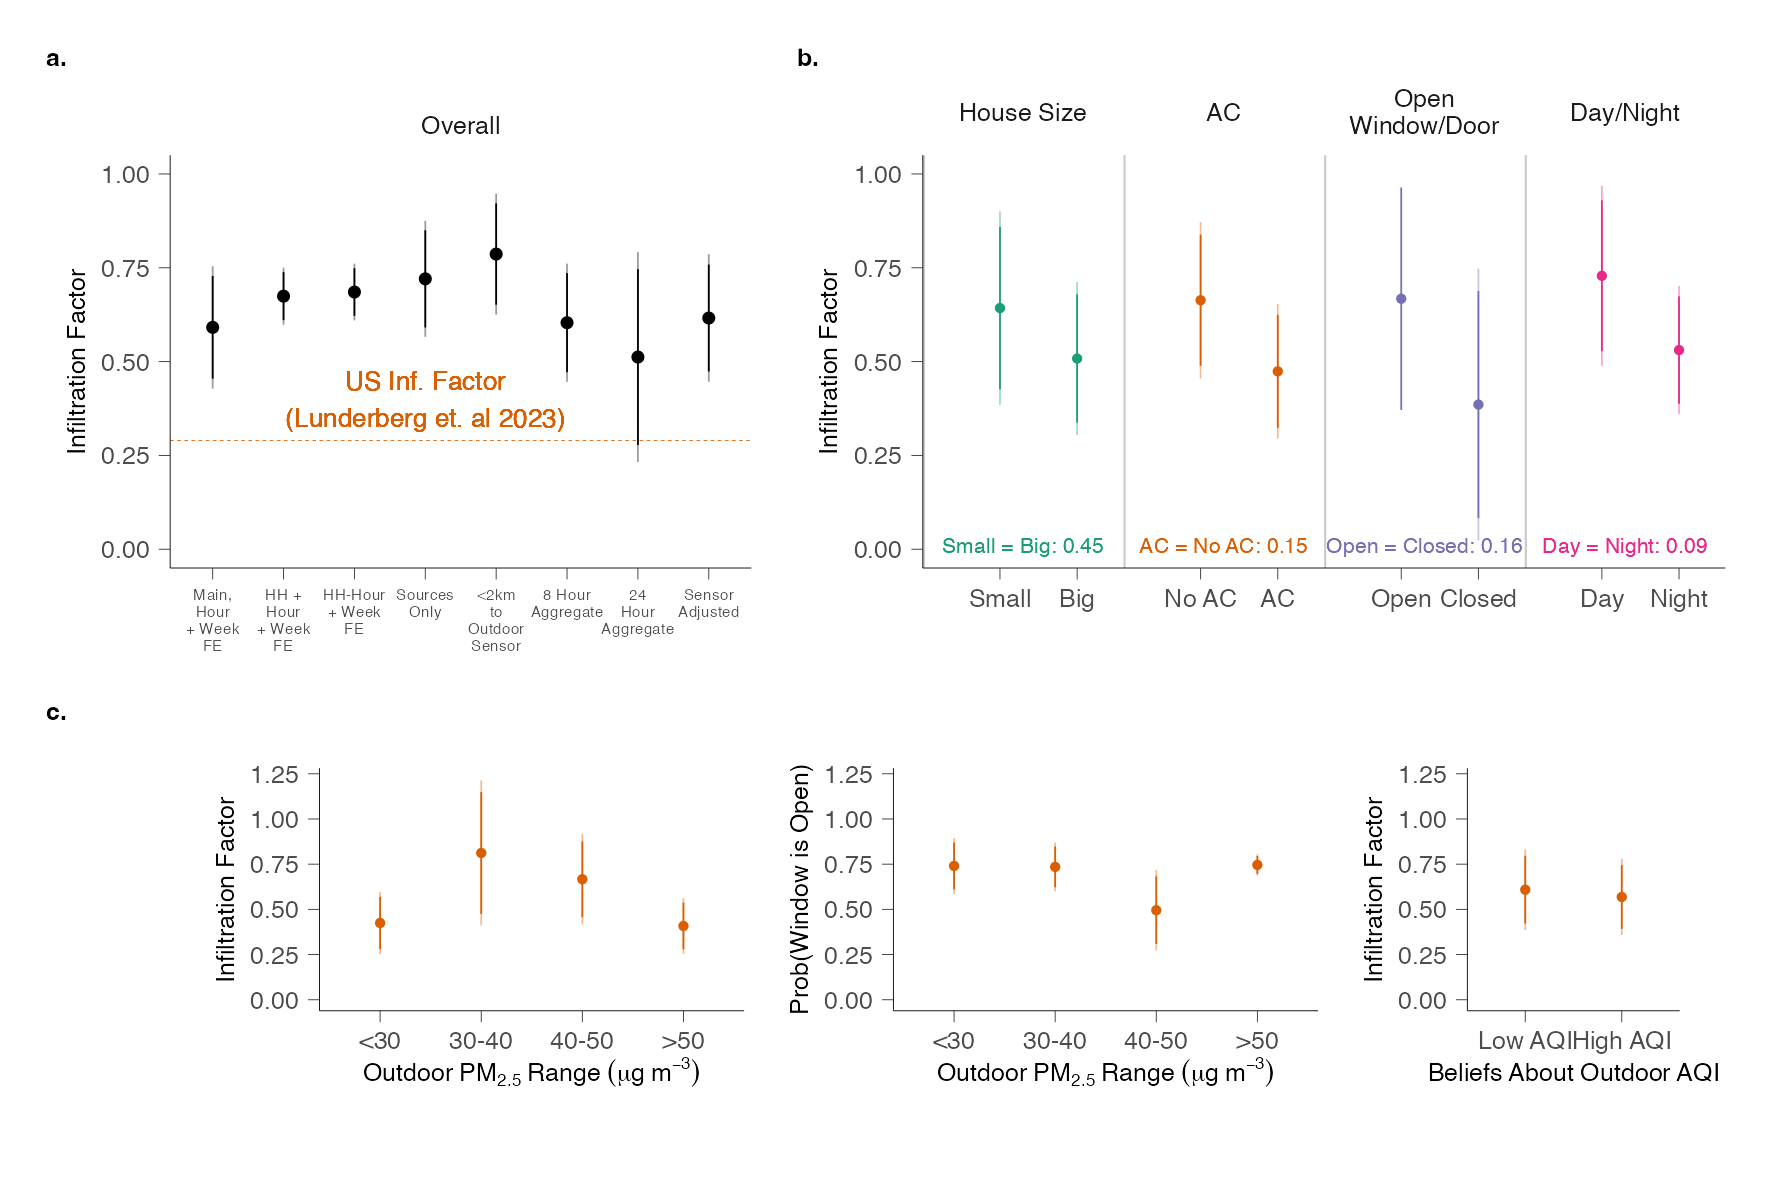
\includegraphics[width=.9\linewidth]{output_clean/figures/fig2_infiltation.png}
    \caption*{\scriptsize This figure summarizes the estimated outdoor-to-indoor infiltration factor, its heterogeneity across household characteristics, and the lack of short-run behavioral responses to higher outdoor pollution. \textbf{(a) Infiltration factors}, defined by the regression of indoor PM$_{2.5}$ on outdoor PM$_{2.5}$ (Equation \ref{eq:infiltration}). Each point corresponds to a different specification. Specifications 1--4 use hourly observations and constitute our main specifications. The first specification controls for hyperlocal source variables (waste burning frequency, household smoking, kitchen source presence, cooking activity, and distance to main road), outdoor temperature, humidity, and hour-of-day and week fixed effects. The second and third add household fixed effects and household-by-hour fixed effects, respectively. The fourth restricts the sample to households within 2 km of an outdoor sensor. Specifications 5 and 6 are robustness checks that aggregate the data to 8-hour and 24-hour means, respectively. All regressions control for outdoor temperature and humidity. The hourly specifications use $N = 148{,}939$ household-hours after conditioning on nonmissing covariates and the 24-hour aggregate specification uses $N = 8{,}910$ household-days.  \textbf{(b) Heterogeneity in infiltration factors} by household and behavioral characteristics, including house size, air conditioning (AC) presence, whether a window or door was open, and time of day (day/night). Each regression includes hyperlocal source controls, outdoor temperature, humidity, and hour-of-day and week fixed effects. P-values for tests of equality between coefficients are shown in the respective panels. Whether the window/door was open came from a survey with $N = 453$ observations. \textbf{(c) Household behavior in response to outdoor pollution levels.} The first panel shows heterogeneity in infiltration factors as a function of outdoor PM$_{2.5}$ concentrations, binned into four ranges. The second panel shows the probability of having a window or door open as a function of outdoor PM$_{2.5}$ concentrations. The third panel shows heterogeneity in infiltration factors based on households' baseline beliefs about whether outdoor air quality is unhealthy (high AQI) versus not (low AQI). Points represent regression coefficients; darker error bars show 90\% confidence intervals, and lighter error bars show 95\% confidence intervals. Errors are clustered at the household and date-hour level.}
    \DIFaddendFL \label{fig:infiltration}
\end{figure}

\DIFdelbegin \DIFdel{We model how ambient outdoor $PM_{2.5}$ infiltrates into indoor spaces; this decomposes the contributions of ambient outdoor sources versus hyperlocal sources to indoor pollution. Ambient outdoor }\DIFdelend \DIFaddbegin \DIFadd{To assess the role of ambient outdoor PM$_{2.5}$ in high indoor PM$_{2.5}$ levels, we model the infiltration of the former into indoor spaces, where ambient outdoor }\DIFaddend refers to background \DIFdelbegin \DIFdel{$PM_{2.5}$ }\DIFdelend \DIFaddbegin \DIFadd{PM$_{2.5}$ }\DIFaddend concentrations measured by our citywide sensor network\DIFdelbegin \DIFdel{, while hyperlocal sources---including smoking and neighborhood burning---occur at spatial scales too fine for our outdoor sensors to capture}\DIFdelend .

We estimate \DIFaddbegin \DIFadd{the infiltration factor of ambient outdoor PM$_{2.5}$.
We find }\DIFaddend that a 1 $\mu g /m^{3}$ increase in ambient outdoor \DIFdelbegin \DIFdel{$PM_{2.5}$ }\DIFdelend \DIFaddbegin \DIFadd{PM$_{2.5}$ }\DIFaddend is associated with a \DIFdelbegin \DIFdel{.689 (}\DIFdelend \DIFaddbegin \DIFadd{.59 to .70 $\mu g/m^3$ increase in indoor PM$_{2.5}$ in the same hour (main specification: .59; }\DIFaddend 95\% CI \DIFdelbegin \DIFdel{, 0.508, 0.871}\DIFdelend \DIFaddbegin \DIFadd{[0.43, 0.75]}\DIFaddend ; $P < 0.001$)\DIFdelbegin \DIFdel{$\mu g /m^{3}$ increase in indoor $PM_{2.5}$ in the same hour. This rate is about 2.5 times the rate }\DIFdelend \DIFaddbegin \DIFadd{, as seen in Fig.\ \ref{fig:infiltration}a. 
These numbers are 2 to 3 times the infiltration factor }\DIFaddend typically estimated in the United States \DIFdelbegin \DIFdel{\citep{lunderberg_assessing_2023}, consistent with indoor spaces in }\DIFdelend \DIFaddbegin \DIFadd{\citep{burke_exposures_2022, lunderberg_assessing_2023} and are broadly consistent with existing evidence from }\DIFaddend low- and middle-income \DIFdelbegin \DIFdel{countries not offering the same protection from outdoor pollution as in high-income countries. In addition, we find that infiltration happens much more quickly }\DIFdelend \DIFaddbegin \DIFadd{settings, where estimates are scarcer }\DIFaddend than in high-income settings \DIFdelbegin \DIFdel{. We estimate that all infiltration happens }\DIFdelend \DIFaddbegin \DIFadd{and often come from studies covering a small number of homes or short monitoring periods.
}

\DIFadd{We also estimated a distributed lagged model, showing that infiltration is happening }\DIFaddend within the hour \DIFdelbegin \DIFdel{, }\DIFdelend \DIFaddbegin \DIFadd{(\textit{SI Appendix}, Fig.\ S1), }\DIFaddend as opposed to estimated lagged effects up to 6 hours in high-income settings \citep{burke_exposures_2022, lunderberg_assessing_2023}. \DIFdelbegin \DIFdel{These estimates are robust to alternative regression models, as seen in Figure \ref{fig:infiltration}a. 
}\DIFdelend \DIFaddbegin \DIFadd{While many studies use daily or multi-hour averaged concentrations to approximate steady-state conditions and to absorb lagged dynamics between outdoor and indoor PM$_{2.5}$ \citep{chen_review_2011}, our distributed lag model results indicate that the outdoor-indoor relationship is essentially contemporaneous in our setting, justifying the use of hourly observations. In Fig.\ \ref{fig:infiltration}a, we show that the estimated infiltration factor is robust to 8-hour (.60, 95\% CI [0.44, 0.76]; $P < 0.001$) and 24-hour (.51, 95\% CI [0.24, 0.78]; $P < 0.001$) aggregations. We note that aggregating to 24-hour means substantially reduces the effective sample size and increases standard errors, because we were unable to collect continuous data for every single hour for all households; results are nevertheless robust to alternative weighting schemes discussed in the Methods (Section \ref{sec:methods}\ref{ssec:methods_sampling} and \textit{SI Appendix}, Fig.\ S2 and S3). 
}\DIFaddend 

\DIFdelbegin \DIFdel{As a result of these high infiltration rates, most indoor air pollution in Jakarta originates from the outdoors---unlike in high-income countries, where indoor pollution typically stems from indoor sources \citep{metcalfe_making_2025}. Overall, we estimate that 63\% of mean indoor PM2.5 comes from ambient outdoor pollution (Figure }\DIFdelend \DIFaddbegin \DIFadd{Ambient outdoor PM$_{2.5}$ is measured with error, since sensors cannot capture the hyperlocal conditions at each household. Measurement error would attenuate the estimated infiltration coefficient toward zero, with greater attenuation for households located farther from a sensor. Consistent with this, we show in \textit{SI Appendix}, Fig.\ S4, that the estimated infiltration factor is stable at approximately 0.84 when we restrict to households within 500m, 1km, and 2km of an outdoor sensor, before declining to 0.59 in the full sample. This suggests that our main estimate represents a conservative estimate of the true infiltration factor.
}

\DIFadd{We leverage the breadth of our survey data to examine drivers of variation in the infiltration factor (Fig.\ }\DIFaddend \ref{fig:infiltration}b). 

\DIFdelbegin \DIFdel{To shed light on the causes behind these high infiltration rates, we examine heterogeneity in infiltration rates in Figure \ref{fig:infiltration}c. We find statistically significant }\DIFdelend \DIFaddbegin \DIFadd{Our results suggest that differences in infiltration factors are partly driven by long-term household structural characteristics and in particular ventilation, which influences the air exchange rate \citep{chen_review_2011}. In particular, we find suggestive }\DIFaddend differences based on air conditioning (AC) ownership (p = \DIFdelbegin \DIFdel{0.08}\DIFdelend \DIFaddbegin \DIFadd{0.15}\DIFaddend ) and whether the monitor room has an open versus closed window or door (p = \DIFdelbegin \DIFdel{0.03) . These findings corroborate ventilation as a key determinant of infiltration rates. }\DIFdelend \DIFaddbegin \DIFadd{0.16) during the measurement hour. }\DIFaddend In Jakarta's hot and humid climate, households without AC often rely on natural ventilation, increasing their exposure to outdoor pollution.

\DIFdelbegin \DIFdel{Our results suggest that differences in infiltration rates are driven by long-term household characteristics. This is in contrast to previous studies in }\DIFdelend \DIFaddbegin \DIFadd{In }\DIFaddend high-income settings\DIFdelbegin \DIFdel{finding that infiltration rates }\DIFdelend \DIFaddbegin \DIFadd{, infiltration factors }\DIFaddend are primarily driven by short-term behavioral adjustments \citep{burke_exposures_2022, baquie_know_2024}. We \DIFdelbegin \DIFdel{conduct three analyses to }\DIFdelend \DIFaddbegin \DIFadd{find no evidence of such responses in Jakarta. Three analyses }\DIFaddend show that households are not actively taking short-term actions to reduce infiltration.

First, while previous literature has found that infiltration \DIFdelbegin \DIFdel{rates }\DIFdelend \DIFaddbegin \DIFadd{factors }\DIFaddend decline at high outdoor \DIFdelbegin \DIFdel{$PM_{2.5}$ }\DIFdelend \DIFaddbegin \DIFadd{PM$_{2.5}$ }\DIFaddend concentrations, suggesting that people actively modify their behavior to limit exposure at higher levels of outdoor pollution \citep{burke_exposures_2022,lunderberg_assessing_2023}, we do not find evidence of this relationship in our setting. In fact, infiltration increases at higher \DIFdelbegin \DIFdel{$PM_{2.5}$ }\DIFdelend \DIFaddbegin \DIFadd{PM$_{2.5}$ }\DIFaddend concentrations. This pattern, shown in \DIFdelbegin \DIFdel{Figure \ref{fig:infiltration}d, could be driven by several factors}\DIFdelend \DIFaddbegin \DIFadd{Fig.\ \ref{fig:infiltration}c, could have several drivers}\DIFaddend , including concentration gradients between outdoor and indoor pollution, meteorological conditions correlated with outdoor pollution levels, or the presence of high-emission hyperlocal pollution sources \citep{lunderberg_assessing_2023,macneill_factors_2012}.

Second, we assess whether ventilation behaviors (e.g., opening windows or doors) respond to outdoor pollution levels. If households actively manage infiltration, we would expect them to close windows when pollution is high. However, \DIFdelbegin \DIFdel{Figure \ref{fig:infiltration}d shows no }\DIFdelend \DIFaddbegin \DIFadd{Fig.\ \ref{fig:infiltration}c shows no clear }\DIFaddend relationship between window or door openness and outdoor pollution levels. While opening or closing windows is a short-term behavior that can, in theory, be adapted, \DIFdelbegin \DIFdel{it is difficult to expect households to }\DIFdelend \DIFaddbegin \DIFadd{we may expect that households do not }\DIFaddend keep windows closed in a hot and humid climate like Jakarta, where natural ventilation is important for cooling. 

Finally, we find no evidence that beliefs translate into meaningful protective action. Infiltration \DIFdelbegin \DIFdel{rates }\DIFdelend \DIFaddbegin \DIFadd{factors }\DIFaddend do not differ between households who perceive outdoor air as unhealthy and those who consider it relatively healthy, as shown in \DIFdelbegin \DIFdel{Figure \ref{fig:infiltration}d}\DIFdelend \DIFaddbegin \DIFadd{Fig.\ \ref{fig:infiltration}c}\DIFaddend . Households were classified based on whether they generally thought outdoor air pollution was unhealthy (high AQI vs.\ low AQI) before monitors were installed. The disconnection between beliefs and protective action is consistent with other research finding low protective behavior in low-income settings \citep{greenstone_indoor_2021, chowdhury_misbeliefs_2025}.



\subsection{\DIFaddbegin \DIFadd{Indoor and }\DIFaddend Hyperlocal Sources of Indoor \DIFdelbegin \DIFdel{$PM_{2.5}$ Spikes}\DIFdelend \DIFaddbegin \DIFadd{PM$_{2.5}$}\DIFaddend }

\DIFaddbegin \DIFadd{We leverage our rich panel of PM$_{2.5}$ data and survey to quantify the contribution of different sources of indoor PM$_{2.5}$. With these high infiltration factors, most indoor air pollution in Jakarta originates from the outdoors. Overall, we estimate that 56\% of mean indoor PM$_{2.5}$ comes from ambient outdoor pollution (Fig.\ \ref{fig:hyperlocal_sources}b), a share toward the upper end of estimates reported for high-income countries \citep{lunderberg_assessing_2023}.
}

\DIFaddend While ambient outdoor pollution is the primary driver of persistently high indoor \DIFdelbegin \DIFdel{$PM_{2.5}$ concentrations, we find that hyperlocal sources are responsible for the episodic spikes that lead to extreme pollution levels. Our surveys, as shown in Figure \ref{fig:hyperlocal_sources}, clearly document the }\DIFdelend \DIFaddbegin \DIFadd{PM$_{2.5}$ concentrations, our surveys shed light on the important role of indoor and hyperlocal sources in both average levels and episodic spikes of indoor PM$_{2.5}$. In particular, in Fig.\ \ref{fig:hyperlocal_sources}, we document the clear }\DIFaddend impact of two major sources: indoor smoking and neighborhood waste burning.


\begin{figure}[H]
    \centering
    \caption{\DIFaddbeginFL \DIFaddFL{Source }\DIFaddendFL Contributions \DIFdelbeginFL \DIFdelFL{of Hyperlocal Pollution}\DIFdelendFL \DIFaddbeginFL \DIFaddFL{to Indoor PM$_{2.5}$}\DIFaddendFL }
    \DIFdelbeginFL
    \DIFdelendFL \DIFaddbeginFL 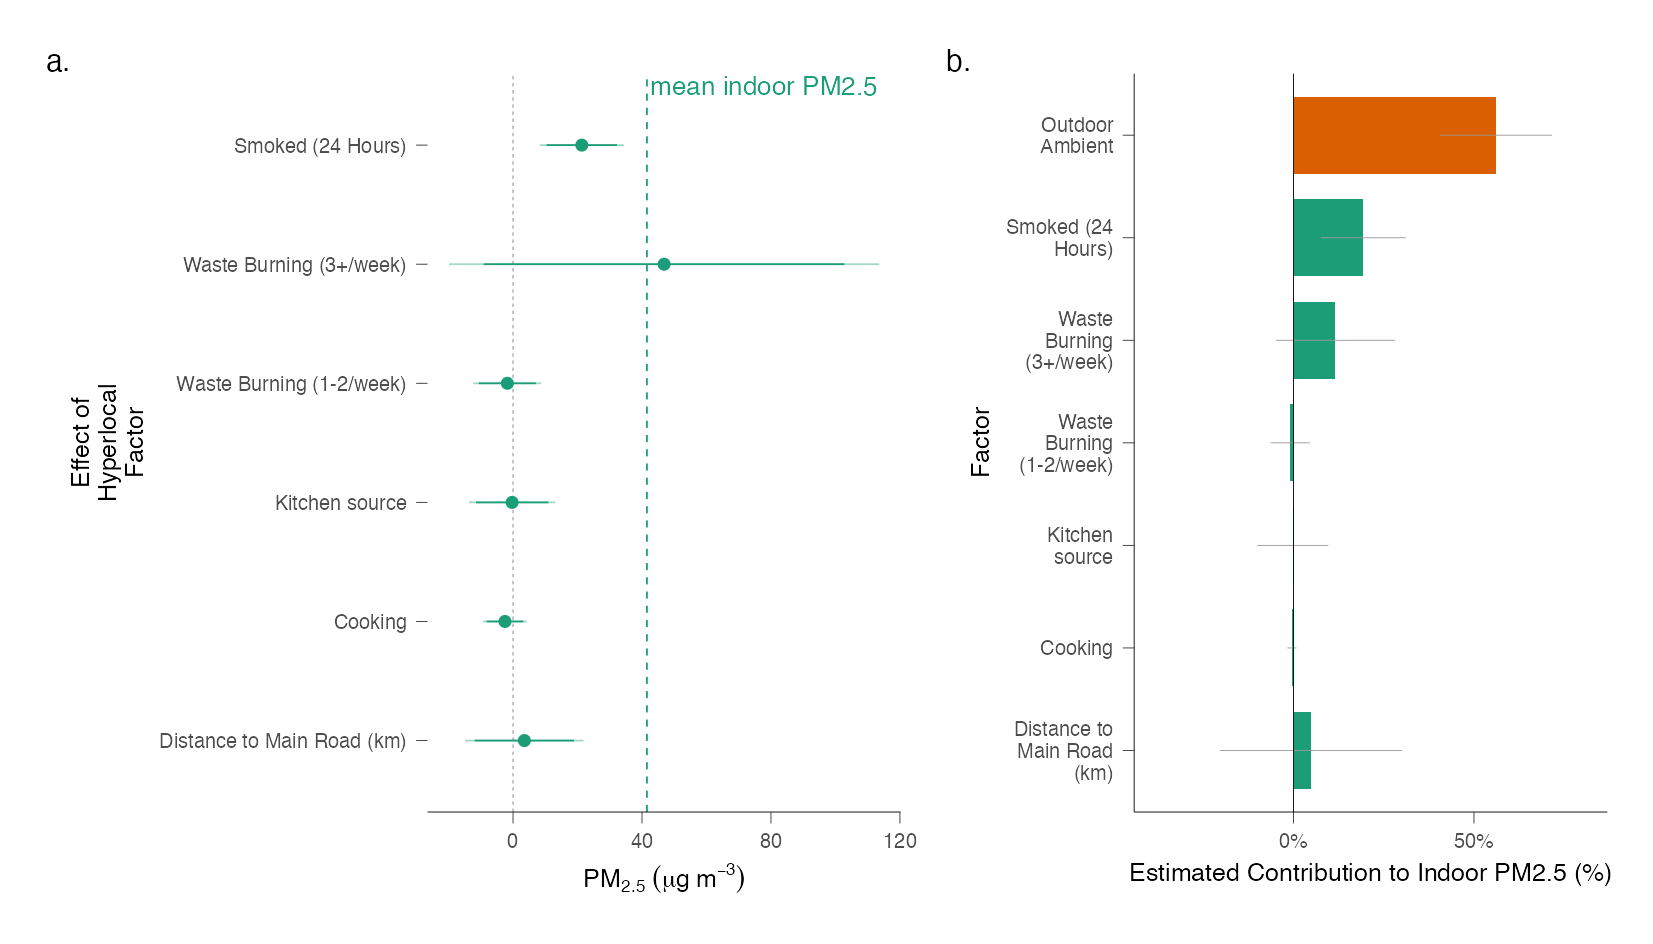
\includegraphics[width=.8\linewidth]{output_clean/figures/fig3_sources.png}
    \caption*{\scriptsize This figure quantifies how ambient outdoor and hyperlocal sources contribute to indoor PM$_{2.5}$ levels. \textbf{(a) Effects of hyperlocal pollution sources on indoor PM$_{2.5}$}, estimated from Equation \ref{eq:infiltration}: whether the household reported any smoking indoors in the 24 hours preceding the interview, whether the household reported observing 1-2 or 3+ waste burning events in the neighborhood in the 7 days preceding the interview, whether the monitor is in or near the kitchen, whether the household was cooking at the time of measurement, and distance to the nearest main road (km). The model controls for outdoor temperature, and humidity, with hour-of-day and week fixed effects. The dashed green line indicates mean indoor PM$_{2.5}$, providing a benchmark against which to interpret the magnitude of each hyperlocal source coefficient. \textbf{(b) Estimated mean contribution of each source to indoor PM$_{2.5}$}, calculated by multiplying each regression coefficient by the sample mean of its corresponding variable and expressing the product as a share of mean indoor PM$_{2.5}$. Panels (a) and (b) use the same sample of 283 households and $N = 148{,}939$ household-hours after conditioning on nonmissing covariates. Error bars are computed by scaling the upper and lower bounds of each coefficient's confidence interval by the sample mean of the corresponding variable and dividing by mean indoor PM$_{2.5}$. Points represent regression coefficients; darker error bars show 90\% confidence intervals, and lighter error bars show 95\% confidence intervals. Standard errors are clustered at the household and date-hour level.}
    \DIFaddendFL \label{fig:hyperlocal_sources}
\end{figure}

We find that households who reported indoor smoking within the last 24 hours experienced significantly higher indoor pollution levels. \DIFdelbegin \DIFdel{These households had a 5.51\% (95\% CI: 1.85--9.17, $P < 0.001$) greater probability of pollution spikes reaching very unhealthy levels. Given that the sample average probability of pollution spikes is 4.43\%, this corresponds to a 127\% increase. Analogously, smoking }\DIFdelend \DIFaddbegin \DIFadd{Smoking }\DIFaddend was associated with \DIFdelbegin \DIFdel{20.8 }\DIFdelend \DIFaddbegin \DIFadd{21 }\DIFaddend $\mu g/m^3$ (95\% CI \DIFdelbegin \DIFdel{: 7.36--34.3, }\DIFdelend \DIFaddbegin \DIFadd{[8.30, 34.4]; }\DIFaddend $P < 0.001$) higher average hourly indoor \DIFdelbegin \DIFdel{$PM_{2.5}$ }\DIFdelend \DIFaddbegin \DIFadd{PM$_{2.5}$ }\DIFaddend concentrations, a \DIFdelbegin \DIFdel{50}\DIFdelend \DIFaddbegin \DIFadd{51}\DIFaddend \% increase compared to the sample mean. \DIFaddbegin \DIFadd{These patterns are remarkably well aligned with global evidence that average measured indoor PM$_{2.5}$ is 20 to 30 $\mu g / m^3$ higher in smoking than non-smoking households \citep{Semple2015}. In our model, smoking explains approximately 19\% of mean indoor PM$_{2.5}$. As a complementary measure of source importance, an LMG R$^2$ decomposition yields a ranking of sources consistent with Fig.\ \ref{fig:hyperlocal_sources} (\textit{SI Appendix}, Table S1).
}\DIFaddend 

Neighborhood-level waste burning is another significant source of indoor air pollution in Jakarta. \DIFdelbegin \DIFdel{Households }\DIFdelend \DIFaddbegin \DIFadd{We estimate that households }\DIFaddend in areas with \DIFdelbegin \DIFdel{more than two }\DIFdelend \DIFaddbegin \DIFadd{at least three }\DIFaddend waste-burning events per week \DIFdelbegin \DIFdel{experienced notably higher indoor $PM_{2.5}$ concentrations}\DIFdelend \DIFaddbegin \DIFadd{(11\% of the sample) experienced higher average indoor PM$_{2.5}$ concentrations; this explains approximately 12\% of the variation in mean indoor PM$_{2.5}$}\DIFaddend . However, accurately quantifying the effect of burning events on indoor pollution is challenging because \DIFdelbegin \DIFdel{we rely }\DIFdelend \DIFaddbegin \DIFadd{of our reliance }\DIFaddend on self-reported data and some events may be misreported. These measurement limitations contribute to wide confidence intervals around our estimates.

\DIFaddbegin \DIFadd{Beyond the difficulty of surveying, waste burning occurs outdoors but at spatial scales finer than our sensor network resolves. Thus it is likely that outdoor sensors partially capture these burn events: households reporting at least three burning events per week have outdoor PM$_{2.5}$ that are 3.65 $\mu g/m^3$ higher on average, increasing to 5.25 $\mu g/m^3$ for households living within 2 km of a sensor (\textit{SI Appendix}, Table S2). This is consistent with evidence that PM$_{2.5}$ from ground-level combustion decays over hundreds of meters \citep{WHO2013REVIHAAP}. However, households reporting frequent burning may also live near other outdoor pollution sources, so we cannot cleanly attribute this differential to waste burning alone. We thus suggest interpreting these estimates with caution.
}


\DIFadd{We additionally examine episodic PM$_{2.5}$ spikes, defined as hours in which the hour-to-hour change in indoor PM$_{2.5}$ exceeds one standard deviation of the overall indoor PM$_{2.5}$ distribution. Episodic spikes are of particular interest because sharp hourly increases are more likely to reflect discrete hyperlocal emission events than the gradual infiltration of ambient outdoor pollution, which varies more smoothly over time. Notably, the probability of an episodic spike was 3.2 percentage points higher in smoking households than in non-smoking households. Smoking is the dominant contributor, accounting for 56\% of the variation in indoor PM$_{2.5}$ spikes, followed by outdoor PM$_{2.5}$ (28\%) and waste burning (24\%). We present a decomposition of source contributions to spikes in \textit{SI Appendix}, Fig.\ S5, mirroring the analysis shown in Fig.\ \ref{fig:hyperlocal_sources}, and the analogous LMG R$^2$ decomposition in \textit{SI Appendix}, Table S3.
}

\DIFaddend In addition to smoking and neighborhood waste burning, there are likely other hyperlocal pollution sources contributing to the observed \DIFaddbegin \DIFadd{levels and episodic }\DIFaddend spikes in indoor air pollution \DIFdelbegin \DIFdel{. Such activities may include cooking, traffic emissions, industrial operations, and commercial activities. An exhaustive list of all polluting activities is beyond the scope of our analysis. }\DIFdelend \DIFaddbegin \DIFadd{but our data is not well suited to draw any conclusive evidence on these. For example, a major contributor to indoor air pollution that has been documented extensively is the combustion of solid fuels and kerosene for cooking. However, in Indonesia, the widespread adoption of LPG cookstoves has largely eliminated variation in cooking fuel use \citep{astuti_successful_2019}; in our survey, 98\% of households reported using LPG cookstoves for cooking. While cooking with LPG cookstoves may still generate large episodic spikes in pollution, our data do not include detailed information on cooking activities, preventing us from drawing insights on this source of indoor pollution. Besides, we do not find that typical cooking hours and whether the air monitor is located in the kitchen impacts measured levels of indoor PM$_{2.5}$ (Fig.\ \ref{fig:hyperlocal_sources}), which may be due partly to the small size and open layout of housing dwellings in our setting. 
Analogously, we find that while distance to a main road is negatively associated with the probability of indoor PM$_{2.5}$ spikes (\textit{SI Appendix} Table S3 and Fig.\ S5a), it does not carry explanatory power on average PM$_{2.5}$ levels (Fig.\ \ref{fig:hyperlocal_sources}), which may reflect the density of Jakarta's road network. For example, 58\% of our sample lives within 500 meters of a main road (\textit{SI Appendix}, Fig.\ S6).
}\DIFaddend 


\subsection{Heterogeneity by Income}

Households across the income distribution experience similar levels of ambient outdoor pollution exposure, but lower-income households \DIFdelbegin \DIFdel{suffer }\DIFdelend \DIFaddbegin \DIFadd{are exposed to }\DIFaddend higher levels of indoor \DIFdelbegin \DIFdel{$PM_{2.5}$. As shown in Figure \ref{fig:pm_income}a, moving }\DIFdelend \DIFaddbegin \DIFadd{PM$_{2.5}$, as displayed in Fig.\ \ref{fig:pm_income}a. Moving }\DIFaddend from the highest to the lowest income quartile in our sample is associated with an increase of \DIFdelbegin \DIFdel{23.4 }\DIFdelend \DIFaddbegin \DIFadd{31.3 }\DIFaddend $\mu g/m^3$ in mean \DIFdelbegin \DIFdel{$PM_{2.5}$, representing a 79\% increase}\DIFdelend \DIFaddbegin \DIFadd{PM$_{2.5}$. Overall, the lowest-income households experience more than double the indoor PM$_{2.5}$ levels of the highest-income households}\DIFaddend . This finding is consistent across various aggregation techniques used to calculate the mean (\DIFdelbegin \DIFdel{SI Appendix, Figure A2}\DIFdelend \DIFaddbegin \DIFadd{\textit{SI Appendix}, Fig.\ S7}\DIFaddend ).

\begin{figure}[H]
    \centering
    \caption{Indoor \DIFdelbeginFL \DIFdelFL{$PM_{2.5}$ }\DIFdelendFL \DIFaddbeginFL \DIFaddFL{PM$_{2.5}$ }\DIFaddendFL Higher for Lower Income Households}
    \DIFdelbeginFL
    \DIFdelendFL \DIFaddbeginFL 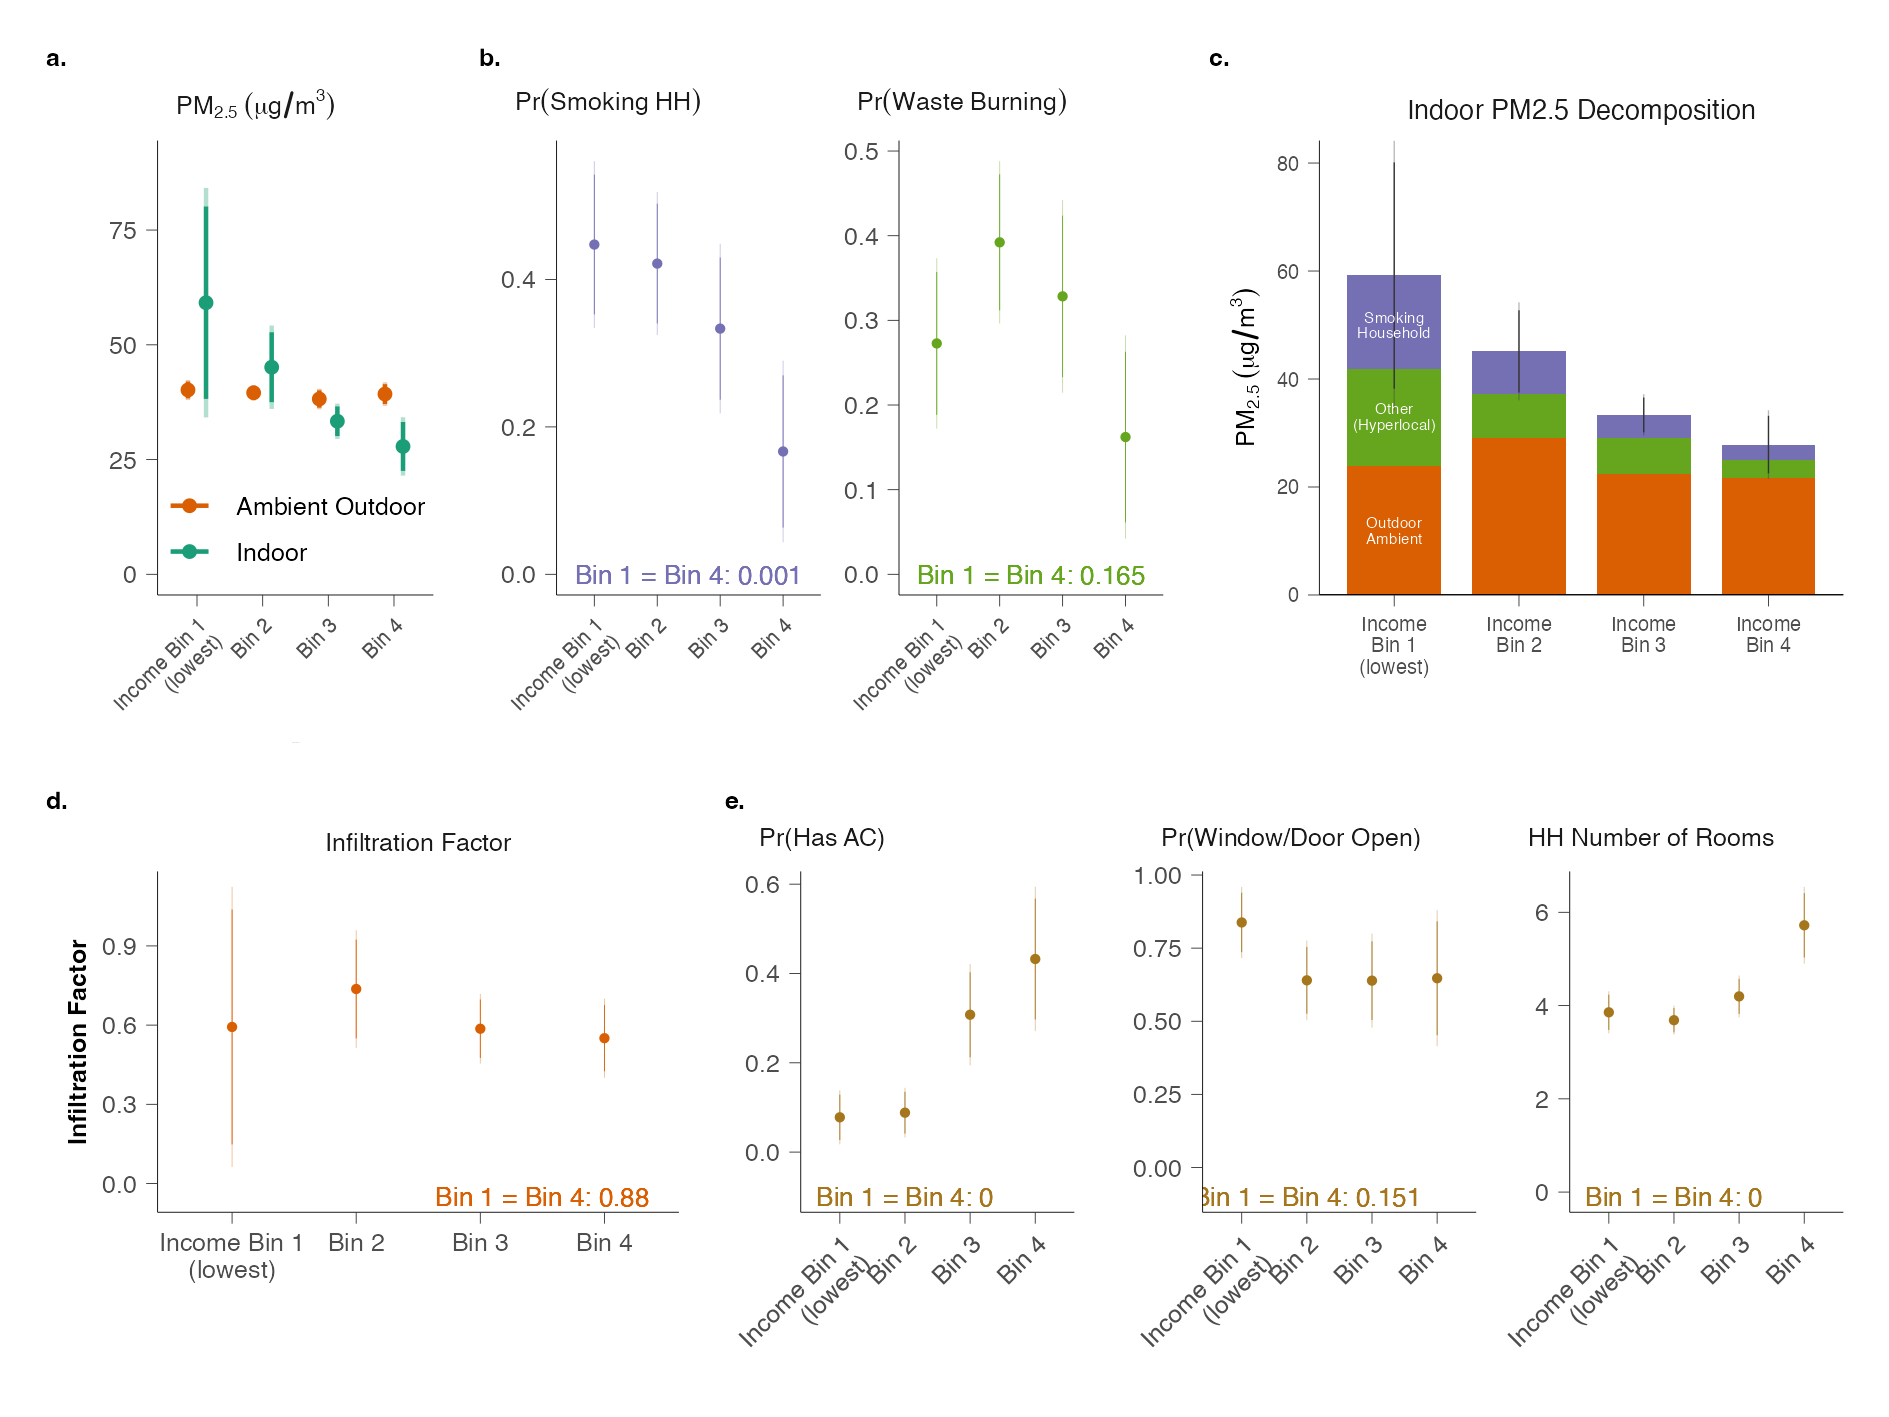
\includegraphics[width=\linewidth]{output_clean/figures/fig4_pm_income.png}
    \caption*{\scriptsize This figure shows how indoor PM$_{2.5}$ and its determinants vary across the income distribution. \textbf{(a) Average indoor and outdoor ambient PM$_{2.5}$ by income quartile.} \textbf{(b) Prevalence of hyperlocal pollution sources by income quartile:} probability of any household member smoking in the past 24 hours, and probability of observing neighborhood waste burning in the past 7 days. 
    \textbf{(c) Decomposition of mean indoor PM$_{2.5}$ by income quartile into outdoor ambient (purple), other hyperlocal sources (orange), and smoking household (green) contributions}. The outdoor ambient contribution is calculated by multiplying income-quartile-specific infiltration factors by quartile-specific mean outdoor PM$_{2.5}$. The smoking contribution is calculated analogously using quartile-specific smoking coefficients and prevalence. The remaining difference is attributed to other hyperlocal sources. \textbf{(d) Infiltration factors by income quartile}, estimated by interacting outdoor PM$_{2.5}$ with income quartile indicators in Equation \ref{eq:infiltration}, controlling for hyperlocal source variables, outdoor temperature, humidity, and hour-of-day and week fixed effects. \textbf{(e) Housing characteristics by income quartile:} probability of having air conditioning, probability of having a window or door open at the time of interview, and number of rooms in the household. Each point is the quartile-specific mean from a regression of the characteristic on income quartile indicators with no intercept. Darker error bars show 90\% confidence intervals, and lighter error bars show 95\% confidence intervals. Standard errors are clustered at the household and date-hour level. P-values for tests of equality between Bin 1 and Bin 4 are shown in panels b, d, and e. Panels (a), (c), and (d) use the 283 households with non-missing indoor PM$_{2.5}$ data and up to $N = 152{,}519$ observed monitor-hours, with smaller regression $N$ where covariates are missing. Panels (b) and (e) use one household survey observation for each of the same 283 households.
}
    \DIFaddendFL \label{fig:pm_income}
\end{figure}

\DIFdelbegin \DIFdel{Indoor air quality is determined by how much outdoor $PM_{2.5}$ infiltrates indoors and how much pollution is generated hyperlocally. }\DIFdelend We find that \DIFdelbegin \DIFdel{income affects both these factors. }\DIFdelend \DIFaddbegin \DIFadd{this heterogeneity in indoor PM$_{2.5}$ exposure across the income spectrum is driven by indoor sources. We estimate that smoking is the biggest driver of this heterogeneity. In Fig.\ \ref{fig:pm_income}b, we show that indoor smoking is significantly less common among higher-income households, translating into a lower contribution of smoking to indoor PM$_{2.5}$ as shown in Fig.\ \ref{fig:pm_income}c. Overall, we estimate that smoking differences explain 45\% of the difference in average indoor PM$_{2.5}$ between the lowest and highest income quartiles.
}\DIFaddend 

\DIFdelbegin \DIFdel{Income may affect infiltration of outdoor pollution into indoor spaces through its impact on housing quality and ventilation choices \citep{lunderberg_assessing_2023}. In Jakarta's hot and humid climate, households may cool indoor spaces through either air conditioning or natural ventilation. As shown in Figure \ref{fig:pm_income}b, higher-income households are significantly more likely to have air conditioning, reducing their reliance on open windows or doors for ventilation. }\DIFdelend \DIFaddbegin \DIFadd{We attribute the remaining 55\% of the difference in average indoor PM$_{2.5}$ between the lowest and highest income quartiles to other hyperlocal factors, rather than differential infiltration of outdoor ambient PM$_{2.5}$. Given the imprecision of these estimates, we do not decompose this residual further. }\DIFaddend Consistent with this \DIFdelbegin \DIFdel{pattern, households in the lowest income quartile are more likely to keep windows or doors open in the air quality monitor room at the time of surveying, although this difference is not statistically significant. Higher-income households also tend to live in larger homes, potentially enabling them to separate living areas from cooking and smoking areas, for example. Taken together, these patterns }\DIFdelend \DIFaddbegin \DIFadd{interpretation, however, we find that waste burning is about half as likely to be reported by participants in the highest income quartile than other participants, though measurement challenges limit the robustness of this finding (Fig.\ \ref{fig:pm_income}b). While cooking fuel combustion has been documented as another major contributor to indoor air pollution, the near-universal adoption of LPG cookstoves in our sample largely eliminates variation in cooking fuel use, limiting our ability to further investigate this channel. We note that high-income households' greater number of rooms and prevalence of AC (Fig.\ \ref{fig:pm_income}e) }\DIFaddend are consistent with \DIFdelbegin \DIFdel{lower-income households having lower housing quality and facing greater challenges in regulating indoor temperatures, making them more vulnerable to outdoor pollution infiltration, as discussed in Section \ref{ssec:infiltration}}\DIFdelend \DIFaddbegin \DIFadd{lower indoor PM$_{2.5}$ concentration, though the remaining 55\% likely reflects a combination of unobserved pollution sources, housing characteristics, and behaviors that we cannot separately identify}\DIFaddend .

\DIFdelbegin \DIFdel{Income is also closely linked to }\DIFdelend \DIFaddbegin \DIFadd{The heterogeneity of indoor and }\DIFaddend hyperlocal pollution sources \DIFdelbegin \DIFdel{shaped by household and neighborhood behaviors. We proxy for exposure to hyperlocal sources by the likelihood that mean hourly $PM_{2.5}$ exceeds the EPA's AQI threshold for very unhealthy levels ($125~\mu g / m^3$}\DIFdelend \DIFaddbegin \DIFadd{across the income gradient is also consistent with a greater burden of episodic pollution for low-income households. We find that households in the lowest income quartile experience PM$_{2.5}$ spikes (defined as hours in which the hour-to-hour change in indoor PM$_{2.5}$ exceeds one standard deviation of the overall indoor PM$_{2.5}$ distribution) 3\% of the time, compared to just 0.4\% for households in the highest income quartile, a statistically significant difference ($p = 0.021$}\DIFaddend ). Since ambient outdoor pollution rarely reaches such extreme \DIFdelbegin \DIFdel{levels }\DIFdelend \DIFaddbegin \DIFadd{jumps }\DIFaddend in Jakarta, these spikes likely result from \DIFaddbegin \DIFadd{more frequent }\DIFaddend episodic emissions occurring inside or near the home\DIFdelbegin \DIFdel{. 

As shown in Figure \ref{fig:pm_income}c, households in }\DIFdelend \DIFaddbegin \DIFadd{, which may be affected by behaviors.
}

\DIFadd{We do not find statistically significant heterogeneity in infiltration rates by income (Fig.\ \ref{fig:pm_income}d). Note that }\DIFaddend the \DIFdelbegin \DIFdel{lowest income quartile experience unhealthy pollution spikes 10.5\% of the time, compared to just 3.23\% in the highest income quartile. A statistical test of the difference in coefficients between the }\DIFdelend \DIFaddbegin \DIFadd{higher prevalence of indoor sources among lower-income households complicates inference: in a mass-balance framework, natural ventilation both increases outdoor infiltration and dilutes indoor emissions, and these opposing forces may mask true differences in infiltration across the income distribution.
}

\section{Discussion}


\DIFadd{We show that indoor PM$_{2.5}$ exposure in the world's most populated city is persistently high, exceeding the WHO 24-hour guideline ($15~\mu g/m^3$) on 78\% of monitored days. While high indoor levels are primarily driven by infiltration from ambient outdoor PM$_{2.5}$, outdoor concentrations are an imperfect proxy for exposure. Indoor and hyperlocal sources contribute significantly to pollution levels and induce extreme short-term pollution events not captured by outdoor monitors. Despite comparable ambient outdoor PM$_{2.5}$ levels, households in the }\DIFaddend lowest income quartile \DIFdelbegin \DIFdel{and the highest quartile confirms that this difference is statistically significant ($p = 0.027$).
This disparity suggests a greater burden of episodic pollution for low-income households.
}\DIFdelend \DIFaddbegin \DIFadd{experience more than double the indoor PM$_{2.5}$ concentration of those in the highest quartile. This disparity is largely driven by smoking and other indoor sources, with additional evidence suggesting that differences in housing characteristics might also play a role. Neither cooking fuel type nor outdoor concentrations, the proxies commonly used in global health frameworks and epidemiological studies, fully capture these patterns.
}

\DIFadd{We estimate an infiltration factor between 0.59 and 0.70, which is substantially higher than estimates in high-income countries.
This estimate is broadly consistent with, and extends, a growing body of evidence from urban LMIC settings such as Dhaka \citep{Sahaetal2025}, Mumbai \citep{Anandetal2022} and Hong Kong \citep{Hossainetal2021}. This evidence has, to date, been largely constrained by small sample sizes (typically less than 50) and short monitoring windows (typically 24 hours). 
With over 152,000 monitor-hours across 283 homes, together with detailed household surveys, our study offers substantially greater statistical power to characterize the distribution of indoor PM$_{2.5}$, the dynamics of infiltration of outdoor air into indoor spaces, how infiltration depends on housing characteristics and ventilation infrastructure, the contribution of indoor and hyperlocal behaviors on average daily pollution and pollution spikes, as well as their determinants across a socioeconomically diverse urban population. Our estimates are significantly different from high-income settings \citep{krebs_using_2021, lunderberg_assessing_2023, burke_exposures_2022}, emphasizing the need for more research in LMIC cities.
}

\DIFadd{This high infiltration factor is likely driven by both a high penetration factor and a high air exchange rate, reflecting the prevalence of natural ventilation and Jakarta's hot and humid climate. Unlike in high-income settings where households reduce infiltration during high pollution episodes by closing windows and using air filtration \citep{burke_exposures_2022}, we find no evidence of such protective behavioral responses in Jakarta. This suggests that avoidance strategies effective in HICs may not transfer to LMIC contexts, where air conditioning is less prevalent and heat limits the ability to keep windows closed.
}

\DIFadd{\textit{SI Appendix}, Table S4 clarifies the mechanisms underlying this pattern using a one-compartment mass-balance model that distinguishes particle entry from ventilation-driven dilution. The framework shows that measures that primarily reduce natural ventilation, such as closing windows or tightening the building envelope, are not uniformly protective. Although reduced ventilation can lower the entry of outdoor pollution, it also limits the dilution of indoor emissions. As a result, in households with substantial indoor sources, particularly households with smokers, these actions can trap indoor PM$_{2.5}$ and increase concentrations. To the extent that indoor sources can be reduced, this would not only lower exposure directly but also expand the scope for net-protective household actions, such as closing windows during outdoor pollution episodes, and for building retrofits. 
}\DIFaddend 

\DIFdelbegin \DIFdel{We further examine the relationship between income and two prominent hyperlocal pollution sources: indoor smoking and neighborhood waste burning. Indoor smoking is significantly less common among higher-income households, as shown in Figure \ref{fig:pm_income}c. Waste burning, another potential contributor, does not follow a clear income gradient, though measurement challenges limit the robustness of this finding. 
}\DIFdelend \DIFaddbegin \DIFadd{The contribution of these indoor sources also raises mismeasurement concerns when ambient outdoor PM$_{2.5}$ is used as a proxy for exposure even though indoor-sourced episodic peaks are not captured by outdoor monitors.
}\DIFaddend 

\DIFdelbegin \section{\DIFdel{Discussion}}

\DIFdel{We show that indoor $PM_{2.5}$ exposure in Jakarta is both persistently high and unequally distributed across income groups.
In addition to elevated average levels, indoor environments frequently experience hazardous pollution spikes}\DIFdelend \DIFaddbegin \DIFadd{Our findings have important distributional implications. Consistent with previous studies \citep{greenstone_indoor_2021, burke_exposures_2022, ito_willingness_2020}, we show that low-income households are exposed to the highest levels of indoor air pollution. 
The socioeconomic gradient in indoor PM$_{2.5}$ concentration is not due to heterogeneous ambient outdoor PM$_{2.5}$ but rather to higher prevalence of indoor and hyperlocal sources among lower-income households. Accurate exposure assessment may therefore require coupling outdoor air quality mapping with demographically representative indoor measurements. This pattern is consistent with recent evidence from London showing that the income gradient in indoor PM$_{2.5}$ can be steeper than the corresponding gradient in ambient outdoor pollution \citep{metcalfe_making_2025}.
}\DIFaddend 

\DIFdelbegin \DIFdel{---extremes not captured by outdoor monitors. These spikes occur despite 98\% of households in our sample using LPG cookstoves---a fuel typically classified as clean cooking.
}\DIFdelend \DIFaddbegin \DIFadd{Importantly, our estimated mean indoor PM$_{2.5}$ of $42.3~\mu g/m^3$---above both the WHO 24-hour ($15~\mu g/m^3$) and annual ($5~\mu g/m^3$) guideline values---is substantially lower than in biomass-dominated settings like Dhaka ($\sim 190~\mu g/m^3$) \citep{GURLEY201311}, yet higher than LPG-using households in Accra ($\sim 24~\mu g/m^3$) \citep{zhou2011household} and comparable to Lima ($41.1~\mu g/m^3$) \citep{kephart2020indoor}, where outdoor traffic-related pollution rather than cooking is the dominant driver. This pattern, corroborated by recent evidence from Dhaka showing indoor PM$_{2.5}$ nearly equivalent to outdoor levels even in households transitioning away from solid fuels \citep{Sahaetal2025}, underscores that ambient outdoor pollution, rather than fuel type alone, can be a binding constraint on indoor air quality in densely polluted LMIC cities. Taken together, these studies consistently document substantial indoor PM$_{2.5}$ exposure in urban LMIC settings; our contribution is to measure these exposures at scale over longer periods and to quantify heterogeneity, spikes, and inequality within a single megacity.
}

\DIFaddend This highlights the need for a broader framework for understanding indoor air pollution in \DIFdelbegin \DIFdel{low- and middle-income countries}\DIFdelend \DIFaddbegin \DIFadd{these contexts}\DIFaddend . For example, the Global Burden of Disease (GBD) framework defines household air pollution in terms of solid fuel use---a metric that has guided policy and resource allocation globally. However, this definition does not fully capture the indoor pollution risks experienced by urban populations that use cleaner fuels but remain exposed to high ambient and infiltrated pollution\DIFaddbegin \DIFadd{, as well as additional indoor or hyperlocal sources like smoking or waste burning}\DIFaddend . 


\DIFdelbegin \DIFdel{We find that most indoor pollution stems from outdoor $PM_{2.5}$ infiltration, with an infiltration factor (0.689) substantially higher than estimates in high-income countries. These high rates are related to structural characteristics, such as the absence of air conditioning and the dependence on natural ventilation, rather than short-term behavioral responses. While information campaigns may increase awareness of infiltration risks, economic and infrastructural constraints likely limit behavioral adjustments. Mitigation efforts must therefore prioritize  pollution controls at the source, targeting major contributors like vehicular traffic and industrial emissions. In the interim, coupling outdoor air quality mapping with demographically representative indoor measurements can help better characterize true exposure and inform more equitable policy design.
}

\DIFdel{In contrast, episodic peaks in indoor pollution are driven by hyperlocal sources such as indoor smoking and neighborhood waste burning, activities more amenable to individual or local intervention. 
Information campaigns and stronger enforcement against garbage burning could reduce these extreme events and their associated health risks.
}

\DIFdel{Our findings also have important distributional implications. Consistent with previous studies \citep{greenstone_indoor_2021, burke_exposures_2022, ito_willingness_2020}, we show that low-income households are exposed to the highest levels of indoor air pollution. Relying solely on outdoor air quality as a proxy for exposure may systematically underestimate both overall exposure and disparities across income groups. These inequalities stem from both higher infiltration rates, associated with poorer housing conditions, and greater hyperlocal emissions. 
}

\DIFdel{Finally, while our study provides novel insights into indoor $PM_{2.5}$ exposure in a developing urban setting, it }\DIFdelend \DIFaddbegin \DIFadd{Despite these contributions, our study }\DIFaddend has several limitations. First, our sample focuses on  households with elementary school-aged children, and therefore is not fully representative of Jakarta's population. Future research should assess whether similar patterns hold for other demographic groups, particularly groups with heightened health risks, such as the elderly or those with pre-existing health conditions. Second, \DIFaddbegin \DIFadd{indoor and outdoor PM$_{2.5}$ were measured using different low-cost sensor models for which no published head-to-head evaluation exists. We therefore interpret absolute indoor--outdoor level differences with more caution than results based on temporal co-variation and the stability of the infiltration estimates across specifications. A formal co-location study of the indoor sensors against a reference-grade monitor in Jakarta would strengthen future work. 
}


\DIFadd{Third, }\DIFaddend while we identify key determinants of indoor air quality, we do not capture all possible hyperlocal pollution sources, such as cooking emissions, incense burning, or traffic-related infiltration, nor are we able to track personal exposure outside the home. 
\DIFaddbegin \DIFadd{Additionally, although we do not estimate different infiltration factors across income groups, we observe differences in housing characteristics such as air conditioning and ventilation infrastructure. Observable differences in housing quality may not map one-for-one into reduced-form differences in infiltration because these features affect both the entry of outdoor pollution and the dilution of indoor emissions. Larger samples and more direct measures of airflow and housing characteristics could help clarify these mechanisms.
}\DIFaddend Relatedly, our reliance on stationary indoor monitors limits our ability to account for variations in individual exposure as people move between environments. Expanding real-time monitoring to include wearable sensors and more detailed measurements of indoor pollution sources could provide a fuller picture of exposure risks.


\section{Materials and Methods} \label{sec:methods}

High levels of outdoor air pollution are sustained in Jakarta throughout the whole year, and historically especially high between the months of May and October. We designed the study to cover this high pollution season and conducted it in two successive rounds, with approximately 154 households participating in each round. Round 1 was conducted from 1 June to 28 August 2024, and Round 2 was conducted from 10 September to 10 December 2024. This randomized controlled trial was registered on the AEA RCT registry (Identification No.\ AEARCTR-0013110) and received IRB approval from the University of Chicago (Protocol No.\ IRB23-0310) and from Badan Riset dan Inovasi Nasional (Application No.\ 29012024000032).

Individual respondents consented to the collection of the indoor air quality data and survey data used in this study. Ambient outdoor \DIFdelbegin \DIFdel{$PM_{2.5}$ }\DIFdelend \DIFaddbegin \DIFadd{PM$_{2.5}$ }\DIFaddend data comes from devices monitored by our hardware implementation partner, not associated with private individuals, and therefore without personally identifying information.


\subsection{Study Participants and Datasets}
\label{ssec:methods_sampling}

\paragraph{Study Participants:} Households participating in our study were selected among Jakarta households, through a partnership with the Education Office in Jakarta, which compiled a representative list of Jakarta schools. We randomly sampled households from school rosters and successfully enrolled 308 participants, \DIFdelbegin \DIFdel{285 }\DIFdelend \DIFaddbegin \DIFadd{283 }\DIFaddend of whom successfully installed the hardware, connected to Wi-Fi, and \DIFdelbegin \DIFdel{operationalized the devices for }\DIFdelend \DIFaddbegin \DIFadd{began }\DIFaddend data collection. Therefore, all our participant households have at least one elementary school child. As surveying challenges like low participation and high attrition are common in developing country cities \citep{greenstone_indoor_2021}, our sample strategy was designed to address these challenges and ensure the proper use and return of air quality hardware. By the end of our study, attrition was only \DIFdelbegin \DIFdel{6}\DIFdelend \DIFaddbegin \DIFadd{8}\DIFaddend \%. This attrition rate is consistent with rates typically observed in rural contexts, but is an exceptionally low rate for surveying in urban settings. For instance, \citep{greenstone_indoor_2021}, a paper with a \DIFdelbegin \DIFdel{similar }\DIFdelend \DIFaddbegin \DIFadd{related }\DIFaddend research question conducted in Delhi, reported attrition rates of 19--32\% across their treatment groups. All analyses were conducted in R version 4.3.2.

\DIFdelbegin \DIFdel{Figure \ref{fig:desc_pm}a displays the }\DIFdelend \DIFaddbegin \DIFadd{The }\DIFaddend geographic distribution of participating households \DIFdelbegin \DIFdel{and }\DIFdelend \DIFaddbegin \DIFadd{is displayed in Fig.\ \ref{fig:desc_pm}a, which }\DIFaddend demonstrates the wide coverage across the city. Households in our sample are relatively larger and less wealthy than the average Jakarta household but span a wide range of socioeconomic backgrounds. For more information on how our sample compares to the wider Jakarta population, see \DIFdelbegin \DIFdel{SI Appendix, Table A2}\DIFdelend \DIFaddbegin \DIFadd{\textit{SI Appendix}, Table S5}\DIFaddend .

Following enrollment, the survey enumerators visited households to obtain informed consent and administer a baseline survey. This survey captured household demographic information, housing structure characteristics, and beliefs and behaviors related to indoor and outdoor air pollution. Upon consent, air quality hardware was installed in the home for approximately three months, during which it collected continuous indoor air quality data. Survey questions are listed in the \DIFdelbegin \DIFdel{SI Appendix}\DIFdelend \DIFaddbegin \DIFadd{\textit{SI Appendix}}\DIFaddend .

\paragraph{Indoor \DIFdelbegin \DIFdel{$PM_{2.5}$}\DIFdelend \DIFaddbegin \DIFadd{PM$_{2.5}$}\DIFaddend :} The air quality hardware consisted of a fan equipped with an internal \DIFdelbegin \DIFdel{$PM_{2.5}$ }\DIFdelend \DIFaddbegin \DIFadd{PM$_{2.5}$ }\DIFaddend sensor (Cubic PM2008M) and was installed in each participating household. The sensor measures particulate concentration via an optical light-scattering method, with accuracy specifications based on factory calibration against a GRIMM aerosol spectrometer. 
The sensors were designed to collect \DIFdelbegin \DIFdel{$PM_{2.5}$ }\DIFdelend \DIFaddbegin \DIFadd{PM$_{2.5}$ }\DIFaddend data in real time, with readings not visible to respondents. When connected to Wi-Fi, the devices transmitted data to a remote server at five-minute intervals, which were subsequently aggregated to the hourly level for analysis. The hardware was produced by Nafas, a Jakarta-based air quality technology company.

To incentivize households to keep the hardware on, participants received IDR 35,000 (approximately USD 2) every 30 days, contingent on the hardware being connected to Wi-Fi and operational for an average of 14 hours per day. For households without Wi-Fi or unwilling to use their Wi-Fi for the experiment, dedicated Wi-Fi units were installed. To offset electricity costs, participants received an additional IDR 15,000 (approximately USD 1) every 30 days.

\DIFaddbegin \DIFadd{Wi-Fi connectivity issues led to intermittent data loss; in these cases, enumerators were dispatched to retrieve readings manually. Data coverage averaged 539 hours per household over the 2--3 month monitoring period. However, coverage varied considerably across households: while most contributed sufficient data for analysis, a subset experienced persistent Wi-Fi signal failure that limited retrievable readings to only a few hours. The full distribution of household-level coverage is reported in \textit{SI Appendix}, Fig.\ S2.
}

\DIFadd{To assess whether non-random patterns of missing data affect our estimates, we re-estimate Equation \ref{eq:infiltration} under three alternative inverse-probability weighting schemes. Our main specification does not include weights, which implicitly upweights households for whom we observe more PM$_{2.5}$ readings. As robustness checks, we alternatively weight by the inverse of (i) the household-specific observation rate, upweighting households with more missing data, and (ii) the household-by-hour observation rate, upweighting household-hour cells with more missing data. If missingness were systematically related to the infiltration rate, these reweighting schemes would shift the estimated coefficient. We find stable estimates across weighting schemes, suggesting that our main results are not driven by differential data coverage across hours, households, or their interaction (\textit{SI Appendix}, Fig.\ S3).
}

\DIFaddend \paragraph{Outdoor \DIFdelbegin \DIFdel{$PM_{2.5}$}\DIFdelend \DIFaddbegin \DIFadd{PM$_{2.5}$}\DIFaddend :} Our hardware partner, Nafas, maintains a dense network of low-cost Airly outdoor sensors across the city, each equipped with a Plantower PMS5003 optical light-scattering sensor. Accuracy and network performance follow the manufacturer's factory calibration and Nafas's routine QA/QC procedures. \DIFaddbegin \DIFadd{This sensor has been broadly deployed and is one of the most extensively studied low-cost sensors. It has been shown to have relatively high accuracy against reference instruments with high hourly correlations (R$^2$ typically between 0.80 and 0.95) \citep{Sayahi2019, Zheng2018}, demonstrating strong temporal tracking despite systematic bias in absolute mass concentrations, especially at high levels of humidity.
While there is no published side-by-side evaluation of the PMS5003 and PM2008M, this issue is most consequential for analyses that hinge on absolute indoor--outdoor mass differences. Our main estimates instead rely on temporal co-variation. A constant level bias between sensor types would therefore be less problematic for the infiltration regressions than for absolute level comparisons, whereas time-varying bias correlated with humidity or pollution episodes would remain a limitation. Consistent with this interpretation, the estimated infiltration factor is stable across hourly, 8-hour, and 24-hour aggregation windows and rises when the sample is restricted to households located closer to outdoor sensors, as expected under attenuation from outdoor measurement error. These checks mitigate concern, but they cannot substitute for a formal co-location study.
}

\DIFaddend For each household, we calculate a weighted average of air quality readings from the three nearest outdoor sensors, assigning weights inversely proportional to the distance to each sensor. The 63 outdoor sensors used in this study also capture temperature and humidity data, which we use as controls. The outdoor low-cost sensors were installed prior to our study and were not randomly distributed across space, which could introduce non-randomly distributed measurement error. We test for selection in the location of outdoor sensors by regressing a household's distance to the closest outdoor sensor on recorded indoor \DIFdelbegin \DIFdel{$PM_{2.5}$}\DIFdelend \DIFaddbegin \DIFadd{PM$_{2.5}$}\DIFaddend , recorded outdoor \DIFdelbegin \DIFdel{$PM_{2.5}$ }\DIFdelend \DIFaddbegin \DIFadd{PM$_{2.5}$ }\DIFaddend of this sensor, household income, house size, whether the household owns an AC, household head employment status, and household head education level. We do not find evidence of selection bias on observables, as shown in the \DIFdelbegin \DIFdel{SI Appendix, Table A1}\DIFdelend \DIFaddbegin \DIFadd{\textit{SI Appendix}, Table S6}\DIFaddend .


\paragraph{Natural ventilation behaviors:} To complement our main survey efforts, we deployed a short WhatsApp survey to participating households on three separate occasions during the study period. The survey asked respondents whether the windows and doors in the room housing the indoor monitor had been open or closed during the past hour.


\subsection{Infiltration \DIFdelbegin \DIFdel{Rate}\DIFdelend \DIFaddbegin \DIFadd{Factor}\DIFaddend }

The average indoor infiltration \DIFdelbegin \DIFdel{rate }\DIFdelend \DIFaddbegin \DIFadd{factor }\DIFaddend is defined as the increase in indoor \DIFdelbegin \DIFdel{$PM_{2.5}$ }\DIFdelend \DIFaddbegin \DIFadd{PM$_{2.5}$ }\DIFaddend concentration per unit increase in local ambient outdoor \DIFdelbegin \DIFdel{$PM_{2.5}$ }\DIFdelend \DIFaddbegin \DIFadd{PM$_{2.5}$ }\DIFaddend concentration. To estimate this \DIFdelbegin \DIFdel{rate}\DIFdelend \DIFaddbegin \DIFadd{factor}\DIFaddend , we used a regression model at the monitor-hour level. For each household $i$ in hour $t$, the infiltration \DIFdelbegin \DIFdel{rate }\DIFdelend \DIFaddbegin \DIFadd{factor }\DIFaddend ($\beta$) was estimated using the following specification:

\begin{align}
\label{eq:infiltration}
    PM^{In}_{it} &= \alpha + \beta PM^{Out}_{it}  \DIFaddbegin \\
    &\quad \DIFadd{+ \pi_1 \mathbf{1}[\text{Smoking}]_i } \notag \\ &\DIFadd{\quad+ \pi_2 \mathbf{1}[\text{Waste burning}]_i + \pi_3 \mathbf{1}[\text{Kitchen}]_i } \notag \\ &\DIFadd{\quad + \pi_4 \mathbf{1}[\text{CookingHour}]_t + \pi_5 \text{DistPrimaryRoad}_i } \notag \\ &\DIFadd{\quad+ \psi }\DIFaddend T_{it} + \gamma H_{it} + \mu_h + \mu_w + \varepsilon_{it} \notag
\end{align}

where $PM^{In}_{it}$ and $PM^{Out}_{it}$ denote indoor and outdoor \DIFdelbegin \DIFdel{$PM_{2.5}$ concentrations }\DIFdelend \DIFaddbegin \DIFadd{PM$_{2.5}$ 
concentrations for household $i$ at hour $t$}\DIFaddend , respectively. 
\DIFaddbegin \DIFadd{$\mathbf{1}[\text{Smoking}]$ indicates whether the respondent reported smoking 
inside the home in the 24 hours preceding the survey. 
$\mathbf{1}[\text{Waste burning}]$ is a categorical indicator for self-reported waste burning activity in the neighborhood in the seven days preceding the survey, 
distinguishing no burning events, one to two events, and at least three events. 
$\mathbf{1}[\text{Kitchen}]$ indicates whether the monitor was located in or  adjacent to the kitchen. 
$\mathbf{1}[\text{Cooking hour}]$ is a binary indicator equal to one if, according to a 24-hour time-use recall survey, the household reported cooking during the hour of day corresponding to $t$. 
$\text{DistPrimaryRoad}$ is the household's distance to the nearest main road, defined as a highway or primary road in the OpenStreetMap classification. 
}\DIFaddend $T_{it}$ and $H_{it}$ are \DIFdelbegin \DIFdel{controls for }\DIFdelend contemporaneous outdoor temperature and \DIFdelbegin \DIFdel{humidity. Hour-of-day controls }\DIFdelend \DIFaddbegin \DIFadd{relative 
humidity, respectively. 
}\DIFaddend $\mu_h$ \DIFdelbegin \DIFdel{capture }\DIFdelend \DIFaddbegin \DIFadd{denotes hour-of-day fixed effects, capturing }\DIFaddend diurnal patterns in \DIFaddbegin \DIFadd{both 
ambient }\DIFaddend pollution and household \DIFdelbegin \DIFdel{activities, and week-of-sample controls }\DIFdelend \DIFaddbegin \DIFadd{activity, and }\DIFaddend $\mu_w$ \DIFdelbegin \DIFdel{capture }\DIFdelend \DIFaddbegin \DIFadd{denotes week-of-sample  fixed effects, capturing longer-run }\DIFaddend temporal trends and \DIFdelbegin \DIFdel{broader }\DIFdelend atmospheric conditions.



\DIFdelbegin \DIFdel{Figure \ref{fig:infiltration}a presents the results of this regression model }\DIFdelend \DIFaddbegin \DIFadd{The estimated $\beta$ }\DIFaddend for this main specification and alternative ones \DIFaddbegin \DIFadd{is presented in Fig.\ \ref{fig:infiltration}a}\DIFaddend : 
\begin{enumerate}
    \item Main specification: includes \DIFdelbegin \DIFdel{controls for }\DIFdelend \DIFaddbegin \DIFadd{household-specific controls that account for non-ambient sources, controls for }\DIFaddend average variation in \DIFdelbegin \DIFdel{$PM_{2.5}$ }\DIFdelend \DIFaddbegin \DIFadd{PM$_{2.5}$ }\DIFaddend over the course of the day (hour-of-day fixed effects, $\mu_h$) and average weekly trends (week-of-sample fixed effects, $\mu_w$).
    \item \DIFdelbegin \DIFdel{All controls included in specification 1, }\DIFdelend \DIFaddbegin \DIFadd{Controls for average variation in PM$_{2.5}$ over the course of the day (hour-of-day fixed effects, $\mu_h$),  average weekly trends (week-of-sample fixed effects, $\mu_w$), }\DIFaddend as well as \DIFdelbegin \DIFdel{controls for }\DIFdelend time-invariant differences across households ($\mu_i$).
    \item \DIFdelbegin \DIFdel{All controls included in specification 1, as well as controls }\DIFdelend \DIFaddbegin \DIFadd{Controls for average weekly trends (week-of-sample fixed effects, $\mu_w$) and }\DIFaddend for household-specific average variation in \DIFdelbegin \DIFdel{$PM_{2.5}$ }\DIFdelend \DIFaddbegin \DIFadd{PM$_{2.5}$ }\DIFaddend at different times of the day (household-hour-of-day fixed effects, $\mu_{ih}$).
    \item Specification 1 but restricts the sample to households located within \DIFdelbegin \DIFdel{1 }\DIFdelend \DIFaddbegin \DIFadd{2 }\DIFaddend km of a low-cost outdoor sensor to assess the potential impact of measurement error in outdoor \DIFdelbegin \DIFdel{$PM_{2.5}$ }\DIFdelend \DIFaddbegin \DIFadd{PM$_{2.5}$ }\DIFaddend concentrations on infiltration estimates.
    \DIFaddbegin \item \DIFadd{Specification 1, but pollution data is aggregated into 8 hour means. }
    \item \DIFadd{Specification 1, but pollution data is aggregated into 24 hour means. }
\DIFaddend \end{enumerate}

The estimated infiltration \DIFdelbegin \DIFdel{rate }\DIFdelend \DIFaddbegin \DIFadd{factor }\DIFaddend ($\beta$) remains highly stable across all specifications. We chose specification 1 \DIFdelbegin \DIFdel{, which includes hour-of-day and week-of-sample fixed effects, }\DIFdelend as our main specification as it enables us to examine heterogeneity by household-level characteristics, which would not be possible in the presence of household fixed-effects ($\mu_i$). 
\\ 

We further investigate lagged effects of outdoor \DIFdelbegin \DIFdel{$PM_{2.5}$ }\DIFdelend \DIFaddbegin \DIFadd{PM$_{2.5}$ }\DIFaddend with the following specification:
\begin{align}
     PM^{In}_{it} &= \alpha + \sum_{k = 0}^{11}\beta_k PM^{Out}_{it} \DIFaddbegin \\
     &\quad \DIFadd{+ \pi_1 \mathbf{1}[\text{Smoking}]_i } \notag \\ &\DIFadd{\quad + \pi_2 \mathbf{1}[\text{Waste burning}]_i + \pi_3 \mathbf{1}[\text{Kitchen}]_i } \notag \\ &\DIFadd{\quad + \pi_4 \mathbf{1}[\text{CookingHour}]_t + \pi_5 \text{DistPrimaryRoad}_i } \notag \\ &\DIFadd{\quad + \psi T_{it} + }\DIFaddend \gamma H_{it} + \mu_h + \mu_w + \varepsilon_{it} \notag
\end{align}

\DIFdelbegin \DIFdel{We }\DIFdelend \DIFaddbegin \DIFadd{In \textit{SI Appendix}, Fig.\ S1, we }\DIFaddend present the results when including 11 lags (outdoor \DIFdelbegin \DIFdel{$PM_{2.5}$ }\DIFdelend \DIFaddbegin \DIFadd{PM$_{2.5}$ }\DIFaddend at each of the previous 11 hours) and ensure that the results are robust to the inclusion of additional lags. From this regression, we derive an estimate of outdoor-indoor infiltration by calculating the cumulative effect of a 1 $\mu g/m^3$ increase in outdoor concentration on indoor concentration:
\begin{align}
    \beta' = \sum_{k=0}^{11} \beta_k
\end{align}

Infiltration \DIFdelbegin \DIFdel{rates }\DIFdelend \DIFaddbegin \DIFadd{factors }\DIFaddend derived from this lagged regression \DIFaddbegin \DIFadd{(.67 - .7) }\DIFaddend are very similar to our main estimates, consistent with most of the infiltration happening within the first hour, as shown in \DIFdelbegin \DIFdel{Figure }\DIFdelend \DIFaddbegin \DIFadd{Fig.\ }\DIFaddend \ref{fig:infiltration}.
\\

To examine heterogeneity in infiltration \DIFdelbegin \DIFdel{rates }\DIFdelend \DIFaddbegin \DIFadd{factors }\DIFaddend across household characteristics $X_i$, we run the following interacted specification:
\begin{align}
    PM^{In}_{it} &= \alpha + \beta_1 PM^{Out}_{it} + \beta_2 X_i + \beta_3(PM^{Out}_{it} \times X_i) \\ 
    &\quad + \pi\DIFaddbegin \DIFadd{_1 \mathbf{1}[\text{Smoking}]_i } \notag \\
    &\DIFadd{\quad + \pi_2 \mathbf{1}[\text{Waste burning}]_i + \pi_3 \mathbf{1}[\text{Kitchen}]_i } \notag \\ &\DIFadd{\quad + \pi_4 \mathbf{1}[\text{CookingHour}]_t + \pi_5 \text{DistPrimaryRoad}_i } \notag \\ &\DIFadd{\quad + \psi }\DIFaddend T_{it} + \gamma H_{it} + \mu_h + \mu_w + \varepsilon_{it} \notag
\end{align}


\DIFaddbegin \subsection{\DIFadd{Decomposition of Indoor PM$_{2.5}$}}

\DIFadd{To decompose indoor PM$_{2.5}$ concentrations by source for Fig.\ \ref{fig:hyperlocal_sources}, we use the coefficients from Equation \ref{eq:infiltration}. We quantify each source's mean contribution to indoor PM$_{2.5}$ by multiplying the estimated coefficient by the sample mean of the corresponding variable and expressing the product as a share of mean indoor PM$_{2.5}$. 
}

\DIFadd{We further assess source importance by decomposing the $R^2$ of Equation \ref{eq:infiltration} across predictors using the Lindeman-Merenda-Gold (LMG) method (\textit{SI Appendix}, Tables S1 and S3) \citep{lindeman_introduction_1980, gromping_relative_2006}.
}


\DIFadd{To quantify how income explains differences in indoor PM$_{2.5}$ exposure, we estimate a single regression of indoor PM$_{2.5}$ on all source variables interacted with income quartile, controlling for outdoor temperature, humidity, and hour-of-day and week fixed effects. This allows the coefficients on outdoor ambient PM$_{2.5}$ (the infiltration factor) and each hyperlocal source to vary by income quartile. We then decompose mean indoor PM$_{2.5}$ for each quartile into three components: the outdoor ambient contribution, calculated by multiplying the quartile-specific infiltration rate by the quartile-specific mean outdoor PM$_{2.5}$; the smoking contribution, calculated analogously using quartile-specific smoking coefficients and prevalence; and a residual hyperlocal component, computed as the difference between observed mean indoor PM$_{2.5}$ and the sum of the outdoor and smoking contributions.
}

\DIFaddend 

\section*{Acknowledgments}
We are very grateful to those at SMERU Institute, including Athia Yumna for project guidance; Maudita Dwi Anbarani, Wandira Senja Larasati, Selly Numrala, and Dimitri Swasthika for outstanding project management and field implementation. We are also grateful to Marianne Bertrand, Fiona Burlig, Joshua Dean, and Michael Greenstone for helpful comments and suggestions. We acknowledge Nafas for their role in supplying hardware and outdoor air quality data to this project. This research was funded by the Asian Development Bank Institute, King Climate Action Initiative of the Abdul Latif Jameel Poverty Action Lab (JPAL), Becker Friedman Institute's Weiss Fund and Development Economics Research Fund, Stevens Doctoral Program Office at Chicago Booth, and the Rustandy Center for Social Sector Innovation at Chicago Booth for their generous financial support. The funders had no role in study design, data collection and analysis, decision to publish or preparation of the manuscript. This research has been approved by the Institutional Review Board (IRB) at the University of Chicago (Protocol No.\ IRB23-0310).

\bibliographystyle{plainnat}
\bibliography{JakartaPM}

\end{document}